\chapter{面向典型孪生场景的3DGS轻量化表达与优化算法}
\label{ch:lightweight_3dgs}

% ---------------- 开篇引言部分（直接书写，不单独开节） ----------------

随着数字孪生技术的不断深化与工业元宇宙概念的落地，
构建高保真、高实时性的三维虚拟场景已成为智慧机房、智慧实验室等典型室内设备密集型场景下日常巡检、远程监控与沉浸式交互的核心需求。
在本文第三章中，针对此类场景中广泛存在的屏幕、金属机柜等高反光与缺乏纹理的复杂材质，
提出了一种基于（此处请替换为第三章的方法缩写）的改进算法，有效解决了复杂光照条件下的三维重建“质”的问题，大幅提升了孪生场景的视觉保真度与几何精确度。
然而，面向实际的工程落地与系统级应用部署，仅仅追求离线渲染质量的提升是远远不够的。
在数字孪生系统的实际运行周期中，终端用户往往需要通过算力与显存受限的普通终端设备（如轻薄笔记本、移动平板）或标准的 Web 浏览器进行实时的场景漫游。
此时，三维场景表达的“效”——即模型占用的物理存储体积、运行时峰值显存占用以及端侧设备的光栅化渲染帧率），直接决定了该孪生系统能否真正投入生产环境。

三维高斯溅射\cite{kerbl20233d}技术虽然凭借其显式的点云表示方法和极其高效的基于瓦片的并行光栅化渲染管线，
在渲染速度上取得了实质性的突破。
但其极度冗余的高维数据结构与极高的显存消耗，也成为了制约其在端侧大规模部署的致命痛点。
正如本文第三章）的实验数据显示，即便经过多模态几何约束优化，一个典型的机房孪生场景模型依然包含约 5.12 百万个高斯基元，
其峰值显存占用高达 8.2 GB，模型文件体积动辄数百兆字节。

在数据结构上，每一个高斯球不仅需要存储基础的三维空间坐标和不透明度），
还必须携带用于表达各向异性几何形状的三维协方差矩阵参数，
以及用于拟合极度耗费存储空间的、与视角相关的外观属性的高阶球谐函数系数。
这种繁杂的数据量导致在算力与内存受限的移动端或 Web 浏览器中，
直接加载该模型会瞬间打满端侧设备的可用显存，引发程序崩溃或产生不可接受的渲染掉帧与卡顿。

% 插入图：典型密集型孪生场景下的端侧应用痛点示意图
\begin{figure}[htbp]
    \centering
    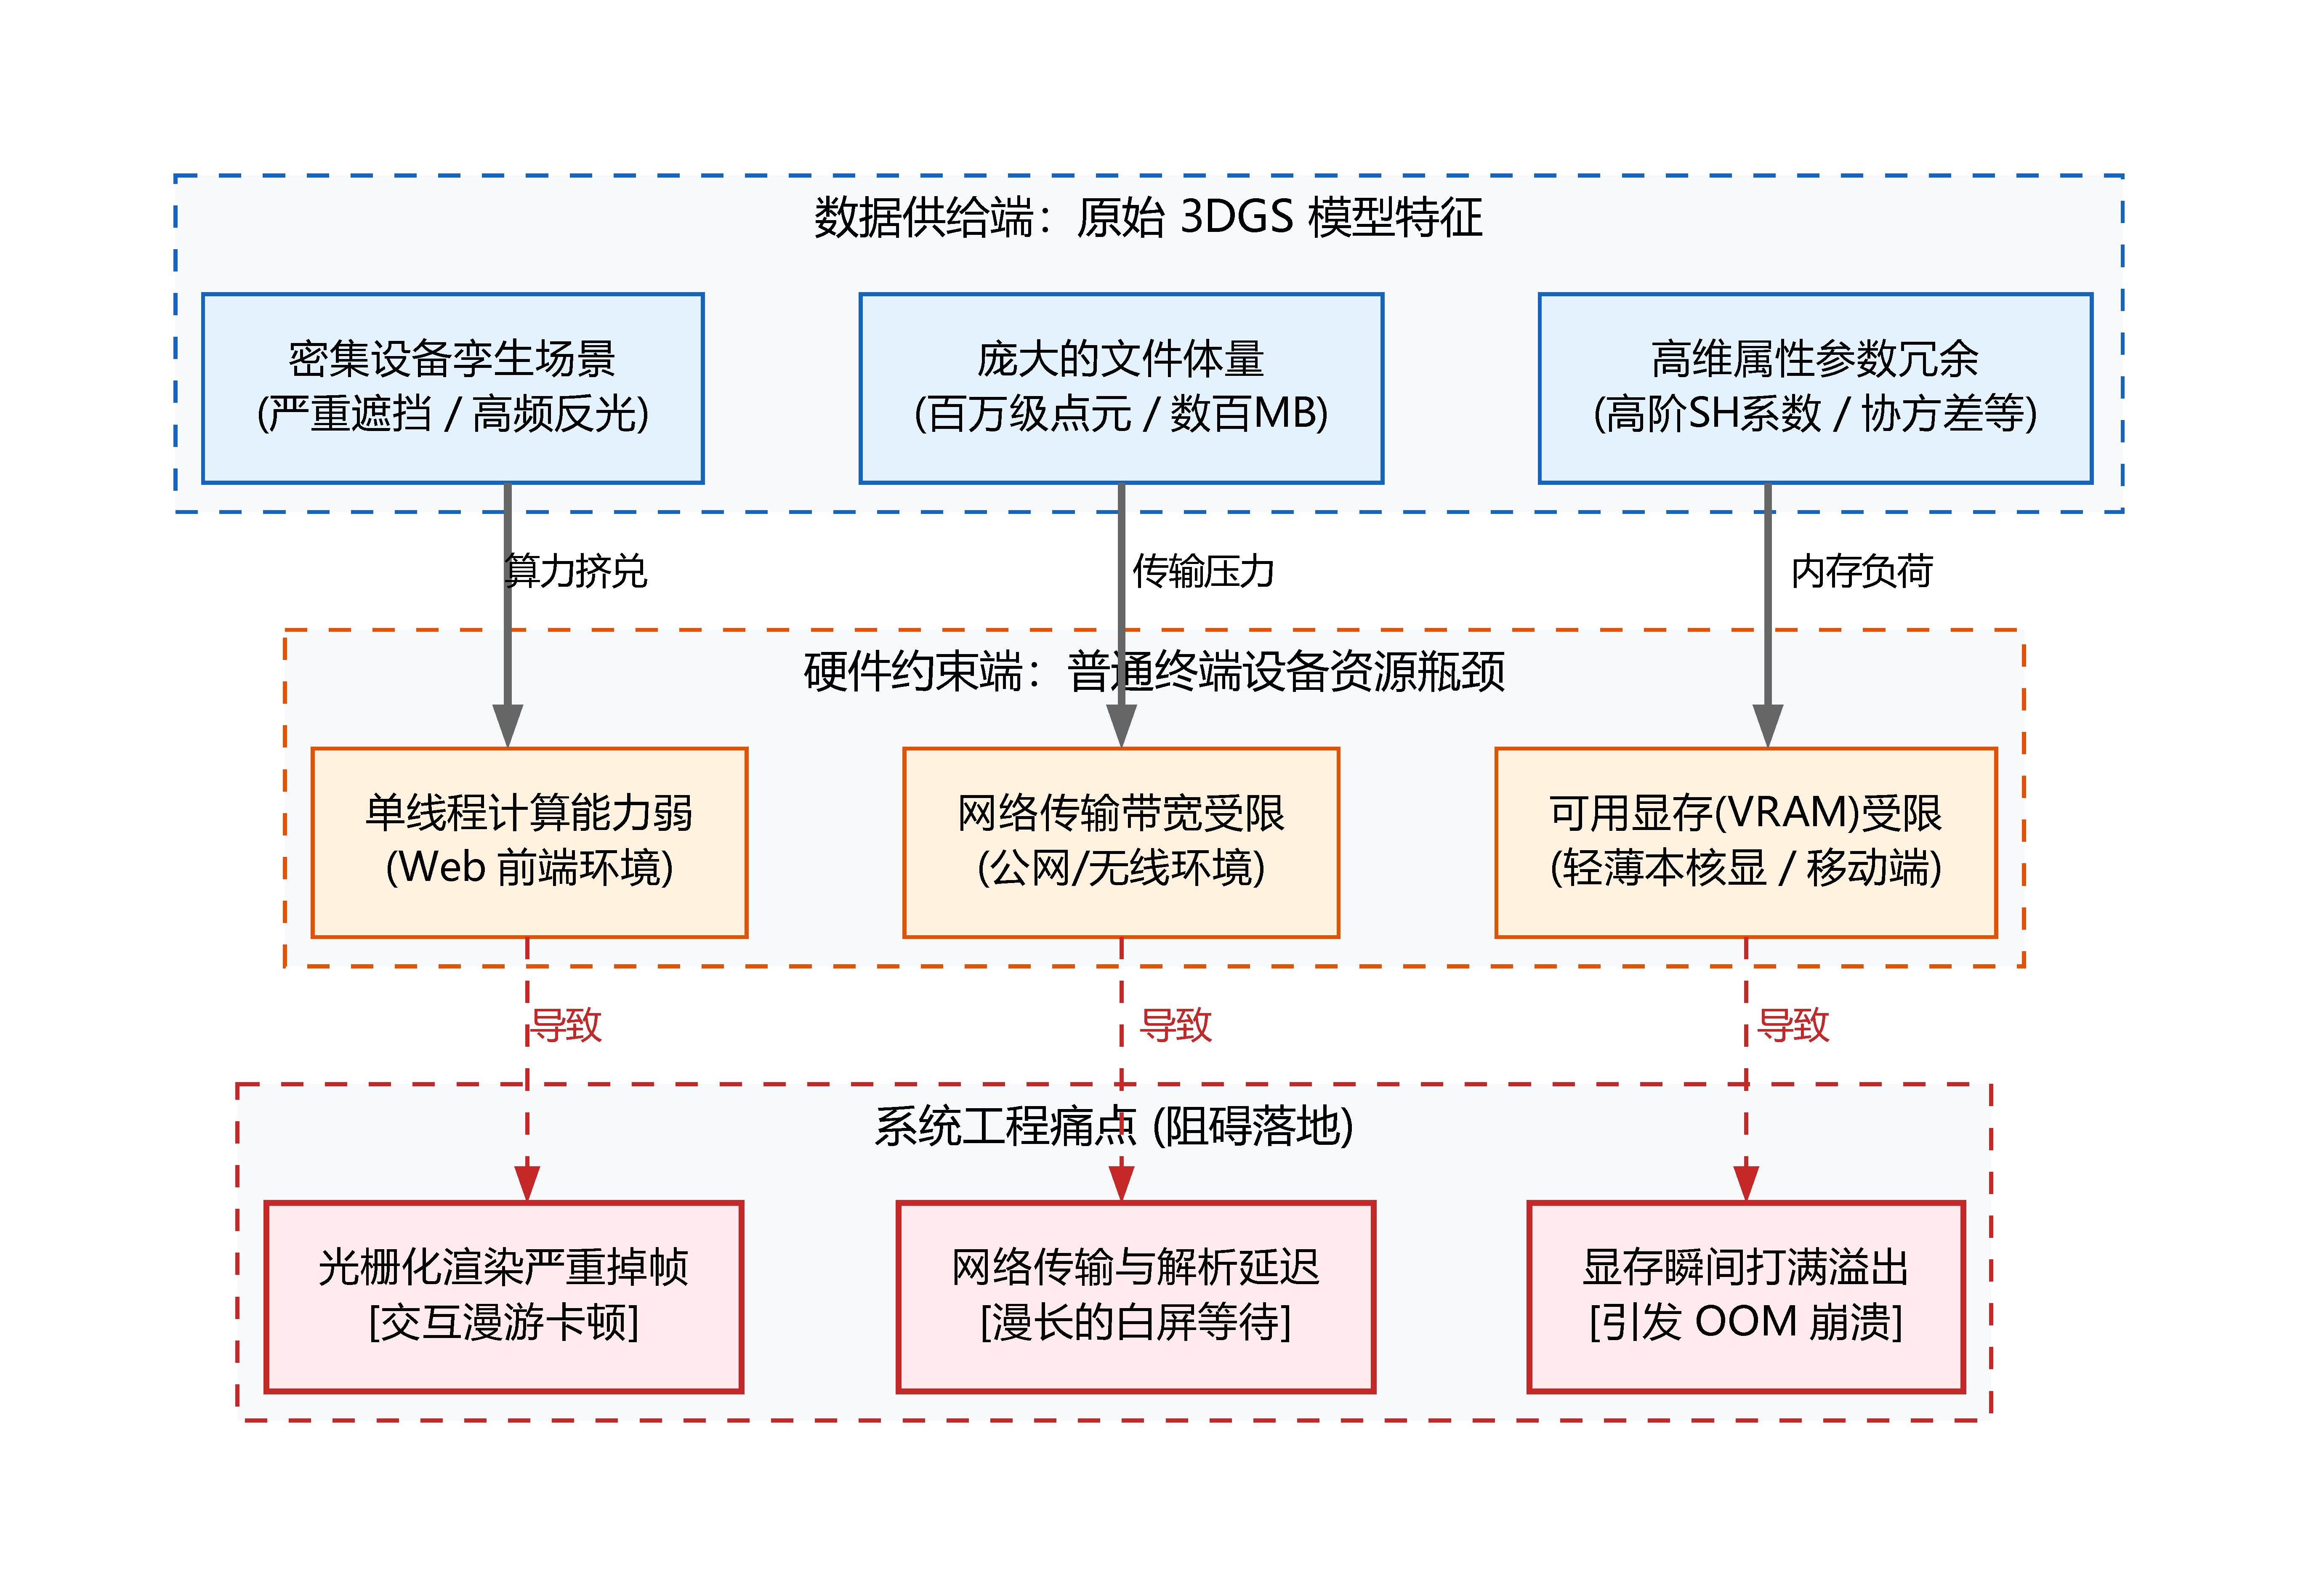
\includegraphics[width=0.85\textwidth]{figures/chap4/fig_4_1_edge_deployment_bottleneck.pdf}
    \caption{典型孪生场景端侧部署痛点：高维数据体量与设备受限算力、带宽之间的矛盾}
    \label{fig:edge_deployment_bottleneck}
\end{figure}


在算力受限的前端设备上直接加载与解析如此庞大的原始 3DGS 模型，
不仅会导致极其漫长的网络传输延迟与系统冷启动耗时，还会瞬间打满端侧设备的可用显存，引发程序崩溃（Out of Memory, OOM）或产生不可接受的渲染掉帧与卡顿。
近年来，尽管学术界陆续涌现出了一些针对 3DGS 的轻量化压缩方案，例如通过网格引导进行下采样的 Compact 3DGS \cite{lee2023compact}，以及引入剪枝与知识蒸馏的 LightGaussian \cite{fan2023lightgaussian}。
但这些通用压缩方法在面对数字孪生机房这种包含密集设备遮挡、精细几何边缘以及第三章所述的复杂高频光影反射场景时，
往往会因为粗暴的参数裁剪或过度的空间离散化，造成不可逆的视觉质量退化（如反光高光细节丢失、设备边缘出现明显的伪影或空洞）。
此外，部分基于复杂熵编码机制的方法 \cite{niedermayr2023compressed} 虽然在理论上大幅降低了存储硬盘体积，
却将计算压力转移到了解码端，引入了巨大的 CPU-GPU 数据解压开销，严重阻碍了端侧的实时渲染流水线。

针对上述理论缺陷与工程应用痛点，本章立足于工业数字孪生系统“降本增效”的实际需求，提出了一种面向典型场景的 3DGS 轻量化表达与端侧渲染优化算法。
该方法致力于在最大限度保持第三章高保真重建质量的前提下，从空间几何冗余剔除、高维属性降维量化以及端侧 Web 渲染管线重构三个维度进行系统性攻关。
本章的主要结构安排如下：第 4.1 节（即下一节）将详细阐述基于多维度重要性评估的冗余高斯精准剔除策略，从几何源头上大幅削减模型的基本体量；
第 4.2 节将深入论述面向高斯球高维参数的矢量量化压缩算法及误差补偿机制；
第 4.3 节探讨高度适配 Web 前端的解码与 Tile-based 渲染调度方案；
第 4.4 节将基于典型场景数据集设计严谨的对比与消融实验，对本章提出算法的多项指标进行全方位验证；最后在第 4.5 节对本章工作进行总结。

\begin{figure}[htbp]
    \centering
    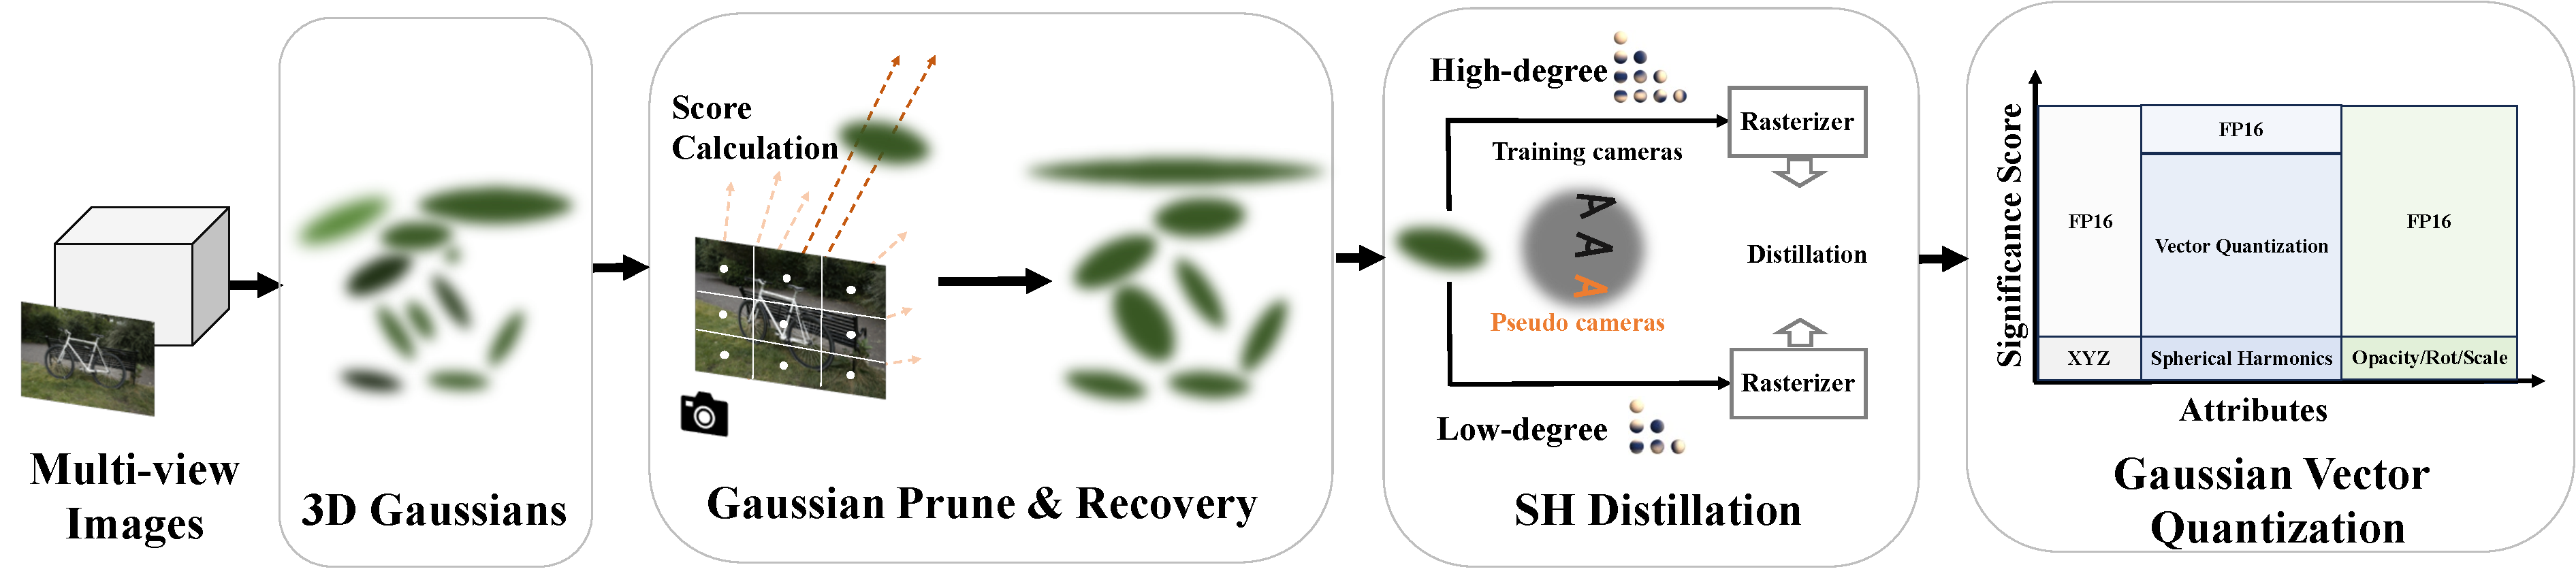
\includegraphics[width=0.96\textwidth]{figures/chap4/fig4_arc.pdf}
    \caption{典型 3DGS 轻量化压缩流程示意图}
    \label{fig:typical_3dgs_compression_pipeline}
\end{figure}

% ---------------- 的第一小节 ----------------

\section{基于重要性评估的冗余高斯剔除策略}
\label{sec:gaussian_pruning}

在面向智慧机房等典型室内孪生场景的三维重建中，
原始 3D Gaussian Splatting (3DGS) 算法虽然能够实现极其逼真的视觉效果，
但其生成的模型通常包含海量的高斯椭球体。
这些高斯体中，有相当一部分对最终的渲染画面几乎没有视觉贡献，却占据了大量的物理存储空间并极大地消耗了端侧设备的渲染显存与内存带宽。
为了从几何数据结构的源头上实现模型的轻量化，
本节深入剖析了 3DGS 算法中高斯点云的生成与演化机理，并提出了一种基于多维度重要性评估的冗余高斯精准剔除（Pruning）策略。

\subsection{3DGS致密化机制与冗余生成机理分析}
\label{subsec:densification_analysis}

要实现精准的几何剔除，首先需要探明冗余高斯球是如何在训练过程中产生的。
3DGS 算法的初始化严重依赖于运动恢复结构（Structure from Motion, SfM）\cite{schonberger2016structure} 算法提取的稀疏特征点云。
然而，在机房、实验室等典型室内场景中，存在大量缺乏纹理的区域（如纯色墙壁、平整的金属机柜表面）以及复杂的设备相互遮挡关系。
在这些区域，SfM 算法往往难以提取到足够密集且准确的特征点，导致 3DGS 的初始点云分布存在大量缺失。

为了弥补初始化点云的不足并强行拟合训练图像的细节，
3DGS 引入了自适应密度控制（Adaptive Density Control, ADC）机制。
在训练的特定迭代周期内，算法会计算每个高斯球在视图空间（View-space）中的二维位置梯度 $\nabla_{\mu_{2D}} L$。
当某个高斯球的位置梯度超过预设阈值 $\tau_{pos}$ 时，表明该区域的重建存在较大误差，算法会触发致密化操作（Densification）。致密化主要包含两种形式：

\begin{enumerate}
    \item \textbf{克隆（Clone）：} 当高斯球体积较小但位置梯度较大时，说明该区域需要更多的几何体来填补空白，算法会在其位置的同一梯度方向上复制生成一个相同的高斯球。
    \item \textbf{分裂（Split）：} 当高斯球体积过大且位置梯度较大时，通常意味着该高斯球试图覆盖过于复杂的几何细节（如跨越了机柜的边缘），算法会将其分裂为两个体积更小的高斯球，其缩放比例通常初始化为原来的 $1/1.6$。
\end{enumerate}

%图 标准 3DGS 单一高斯球内存占用占比饼图
\begin{figure}[htbp]
    \centering
    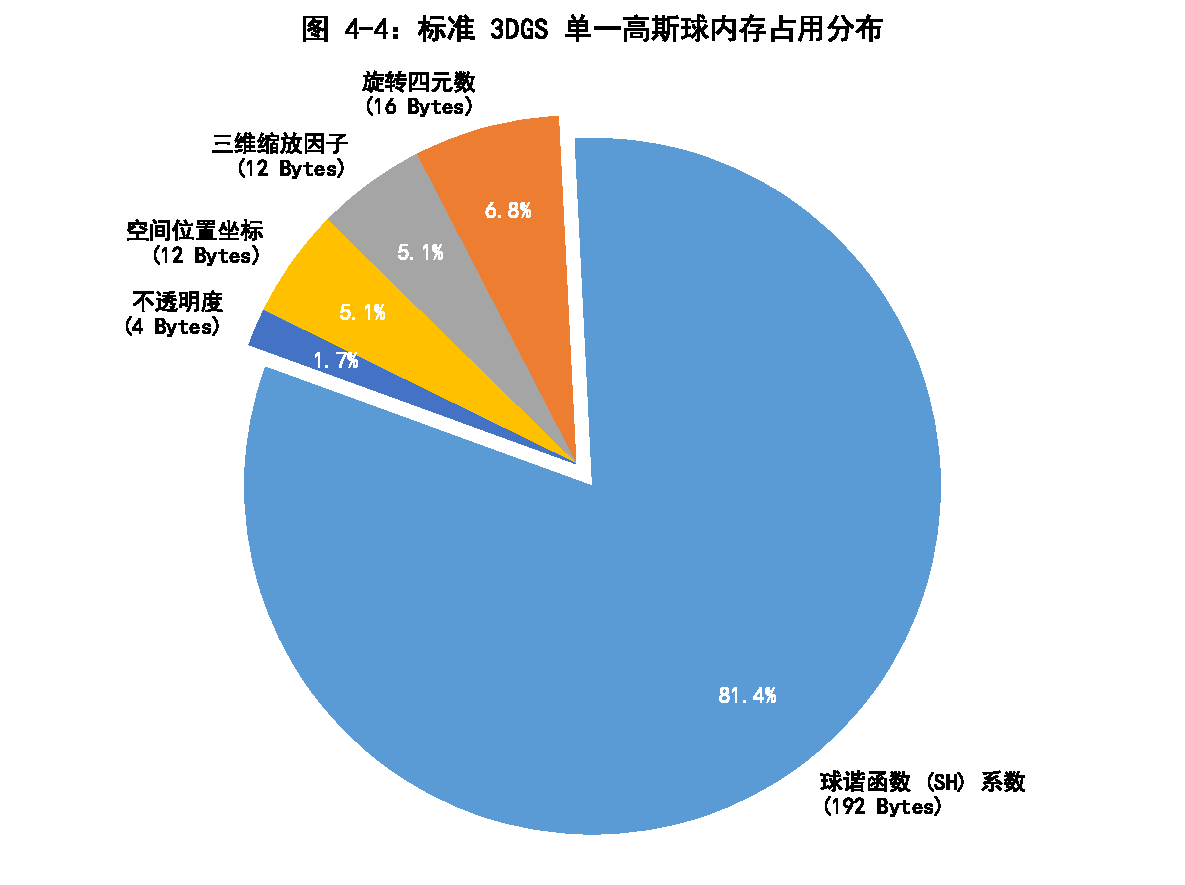
\includegraphics[width=0.75\textwidth]{figures/chap4/fig_4_4_memory_pie.pdf}
    \caption{单高斯球内存占用分布：高维球谐函数（SH）系数占据超过 81\% 的总存储空间}
    \label{fig:memory_footprint}
\end{figure}

尽管 ADC 机制极大地提升了重建的精细度，
但在机房这种存在大面积非朗伯体（Non-Lambertian）高反光表面（如显示器屏幕）和严重遮挡的场景中，梯度优化往往会陷入局部最优。
为了拟合屏幕反光或者遮挡边界的复杂光路，优化器会在墙壁内部、机柜背面等“不可见区域”疯狂地触发分裂和克隆，生成数以百万计的“幽灵高斯”（Ghost Gaussians）。
这些高斯球由于被表层结构完全遮挡，或者自身的不透明度极低，对任意训练视角的有效渲染几乎为零。
这正是我们需要进行几何剪枝的核心目标。

\subsection{多维度高斯重要性评估指标构建}
\label{subsec:importance_metric}

传统的轻量化方法往往仅采用单一的全局不透明度阈值（如剔除所有 $\alpha < 0.005$ 的点）来进行粗暴裁剪。
这种方法在简单场景下尚可，但在光影复杂的机房场景中，极易误删用于拟合微弱高光或半透明边缘的有效高斯球。
为此，本章提出从三个正交的维度构建一个综合重要性评估指标（Comprehensive Importance Metric, $\mathcal{I}$）。

\subsubsection{基于体积渲染方程的有效渲染贡献度}

3DGS 的渲染管线本质上是对传统体积渲染（Volume Rendering）\cite{mildenhall2021nerf} 的离散化近似。
对于相机发出的任意一条射线 $\mathbf{r}$，其最终在屏幕像素上呈现的颜色 $C(\mathbf{r})$ 由沿射线排序的 $N$ 个高斯球混合而成：

\begin{equation}
    C(\mathbf{r}) = \sum_{i=1}^{N} c_i \alpha_i T_i
\end{equation}

其中，$c_i$ 为第 $i$ 个高斯球的颜色，$\alpha_i$ 为其在该射线视角下的计算不透明度。
关键参数 $T_i$ 被称为透射率（Transmittance），表示光线在穿过前 $i-1$ 个高斯球后剩余的能量比例，其计算公式为：

\begin{equation}‘
    ’T_i = \prod_{j=1}^{i-1}(1-\alpha_j)
\end{equation}

从上述公式可以推导出：一个高斯球即便拥有较高的固有不透明度 $\alpha_i$，
如果它始终被排列在前面的高斯球遮挡（即前序的 $\alpha_j$ 接近 1，
导致 $T_i$ 趋近于 0），那么它对最终画面颜色 $C(\mathbf{r})$ 的实际贡献量依然微乎其微。
因此，我们定义高斯球 $i$ 在特定视图 $v$ 下的有效贡献度 $\omega_{i,v}$ 为其在所有穿过该球的射线中的最大累积权重：

\begin{equation}
    \omega_{i,v} = \max_{\mathbf{r} \in \mathcal{R}_v} (\alpha_{i,\mathbf{r}} \cdot T_{i,\mathbf{r}})
\end{equation}

考虑到工业机房通常需要多视角的漫游，
我们将该指标扩展至整个训练视图集合 $\mathcal{V}$，得到全局平均视图可见性权重 $\overline{\omega}_i$：

\begin{equation}
    \overline{\omega}_i = \frac{1}{|\mathcal{V}|} \sum_{v \in \mathcal{V}} \omega_{i,v}
\end{equation}

该权重 $\overline{\omega}_i$ 能够精准且严格地筛选出那些深埋于物体内部、处于视场盲区或被完全遮挡的冗余几何体。

\subsubsection{几何尺度与空间分布惩罚}

除了渲染贡献度，高斯球的物理几何特征同样是判断其是否冗余的重要依据。
在机房场景的重建中，我们观察到两类极端的无用高斯球：第一类是极度细小的“粉尘点”，它们通常是优化过程中的数值噪声；
第二类是体积畸大且呈现极度扁平状（即各向异性极强）的“背景球”，它们试图用极低的透明度覆盖大面积的纯色背景。
设高斯球 $i$ 的三维协方差矩阵对应的三个主轴缩放因子分别为 $s_{i,1}, s_{i,2}, s_{i,3}$，我们定义其固有空间体积 $V_i$ 为：

\begin{equation}
    V_i = s_{i,1} \cdot s_{i,2} \cdot s_{i,3}
\end{equation}

为了惩罚这些极端尺度的几何体，我们引入了基于高斯体积的正则化惩罚项 $\mathcal{P}_{vol}(i)$：

\begin{equation}
    \mathcal{P}_{vol}(i) = \exp\left(-\frac{(V_i - V_{median})^2}{2\sigma_V^2}\right)
\end{equation}

其中 $V_{median}$ 为当前场景中所有高斯球体积的中位数，$\sigma_V$ 为体积分布的标准差。
该惩罚项使得体积过大或过小的高斯球在最终评分中获得较低的权重。

\begin{figure}[htbp]
    \centering
    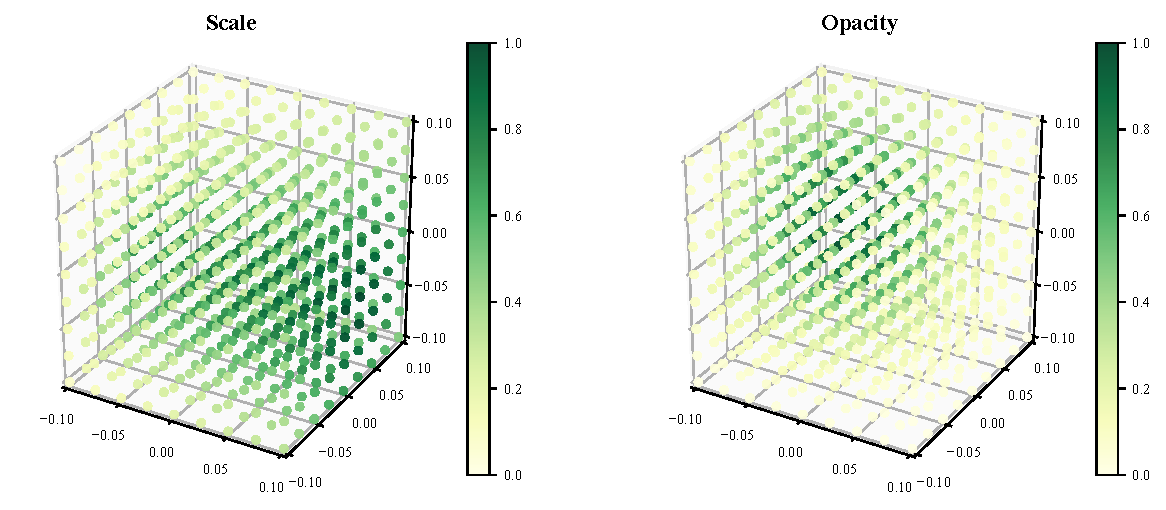
\includegraphics[width=0.82\textwidth]{figures/chap4/fig4_view_adaptive_gaussian_attributes.pdf}
    \caption{视角自适应高斯属性可视化示意图}
    \label{fig:view_adaptive_gaussian_attributes}
\end{figure}



\subsubsection{综合重要性评分函数}

综合上述对有效渲染贡献度 $\overline{\omega}_i$、固有不透明度 $\alpha_i$ 以及几何尺度惩罚 $\mathcal{P}_{vol}(i)$ 的分析，
我们最终构建了面向多维特征的高斯综合重要性评分函数 $\mathcal{I}_i$：

\begin{equation}
    \mathcal{I}_i = \lambda_1 \cdot \overline{\omega}_i + \lambda_2 \cdot \sigma(\alpha_i) \cdot \mathcal{P}_{vol}(i)
\end{equation}

式中，$\sigma(\cdot)$ 为 Sigmoid 激活函数，用于将基础不透明度非线性映射至 $(0, 1)$ 区间；$\lambda_1$ 与 $\lambda_2$ 为平衡渲染权重与几何特征的超参数（在本文的机房场景实验中，依据经验通常设定 $\lambda_1 = 0.7, \lambda_2 = 0.3$）。
通过计算每一个高斯体的 $\mathcal{I}_i$ 评分，我们为后续的自动化剪枝提供了坚实的数学依据。

\subsection{自适应阈值过滤与点云提纯算法}
\label{subsec:adaptive_threshold}

在获取了包含全场景数百万高斯球的评分集合 $\mathcal{I} = \{ \mathcal{I}_1, \mathcal{I}_2, \dots, \mathcal{I}_M \}$ 后，如何设定剔除阈值 $\tau_{prune}$ 成为了决定轻量化效果与视觉质量平衡的关键。
如果采用固定不变的硬阈值，很难适应不同规模和复杂度的机房场景。

本章提出了一种基于统计分布的自适应阈值截断策略。
首先，对整个集合 $\mathcal{I}$ 按得分进行升序排列。
由于冗余高斯球通常占据极大比例且得分集中在极低值区间，其概率密度函数（PDF）呈现出明显的长尾分布（Long-tail Distribution）特征。
我们采用最大类间方差法（Otsu's Method）\cite{otsu1979threshold} 的变体来寻找最优分割点。
具体而言，算法寻找一个阈值 $\tau$，使得被划分为“保留组”和“剔除组”的两类高斯球，其重要性得分的类间方差最大化。
在实际工程实现中，为了保证重建质量的绝对安全下限，我们会在 Otsu 计算结果的基础上叠加一个最大剔除比例限制（例如 $\eta_{max} = 60\%$）。
即，如果自适应阈值导致需要剔除的点数超过了总点数的 60\%，则强制调低阈值以保全几何结构。



\begin{figure}[htbp]
    \centering
    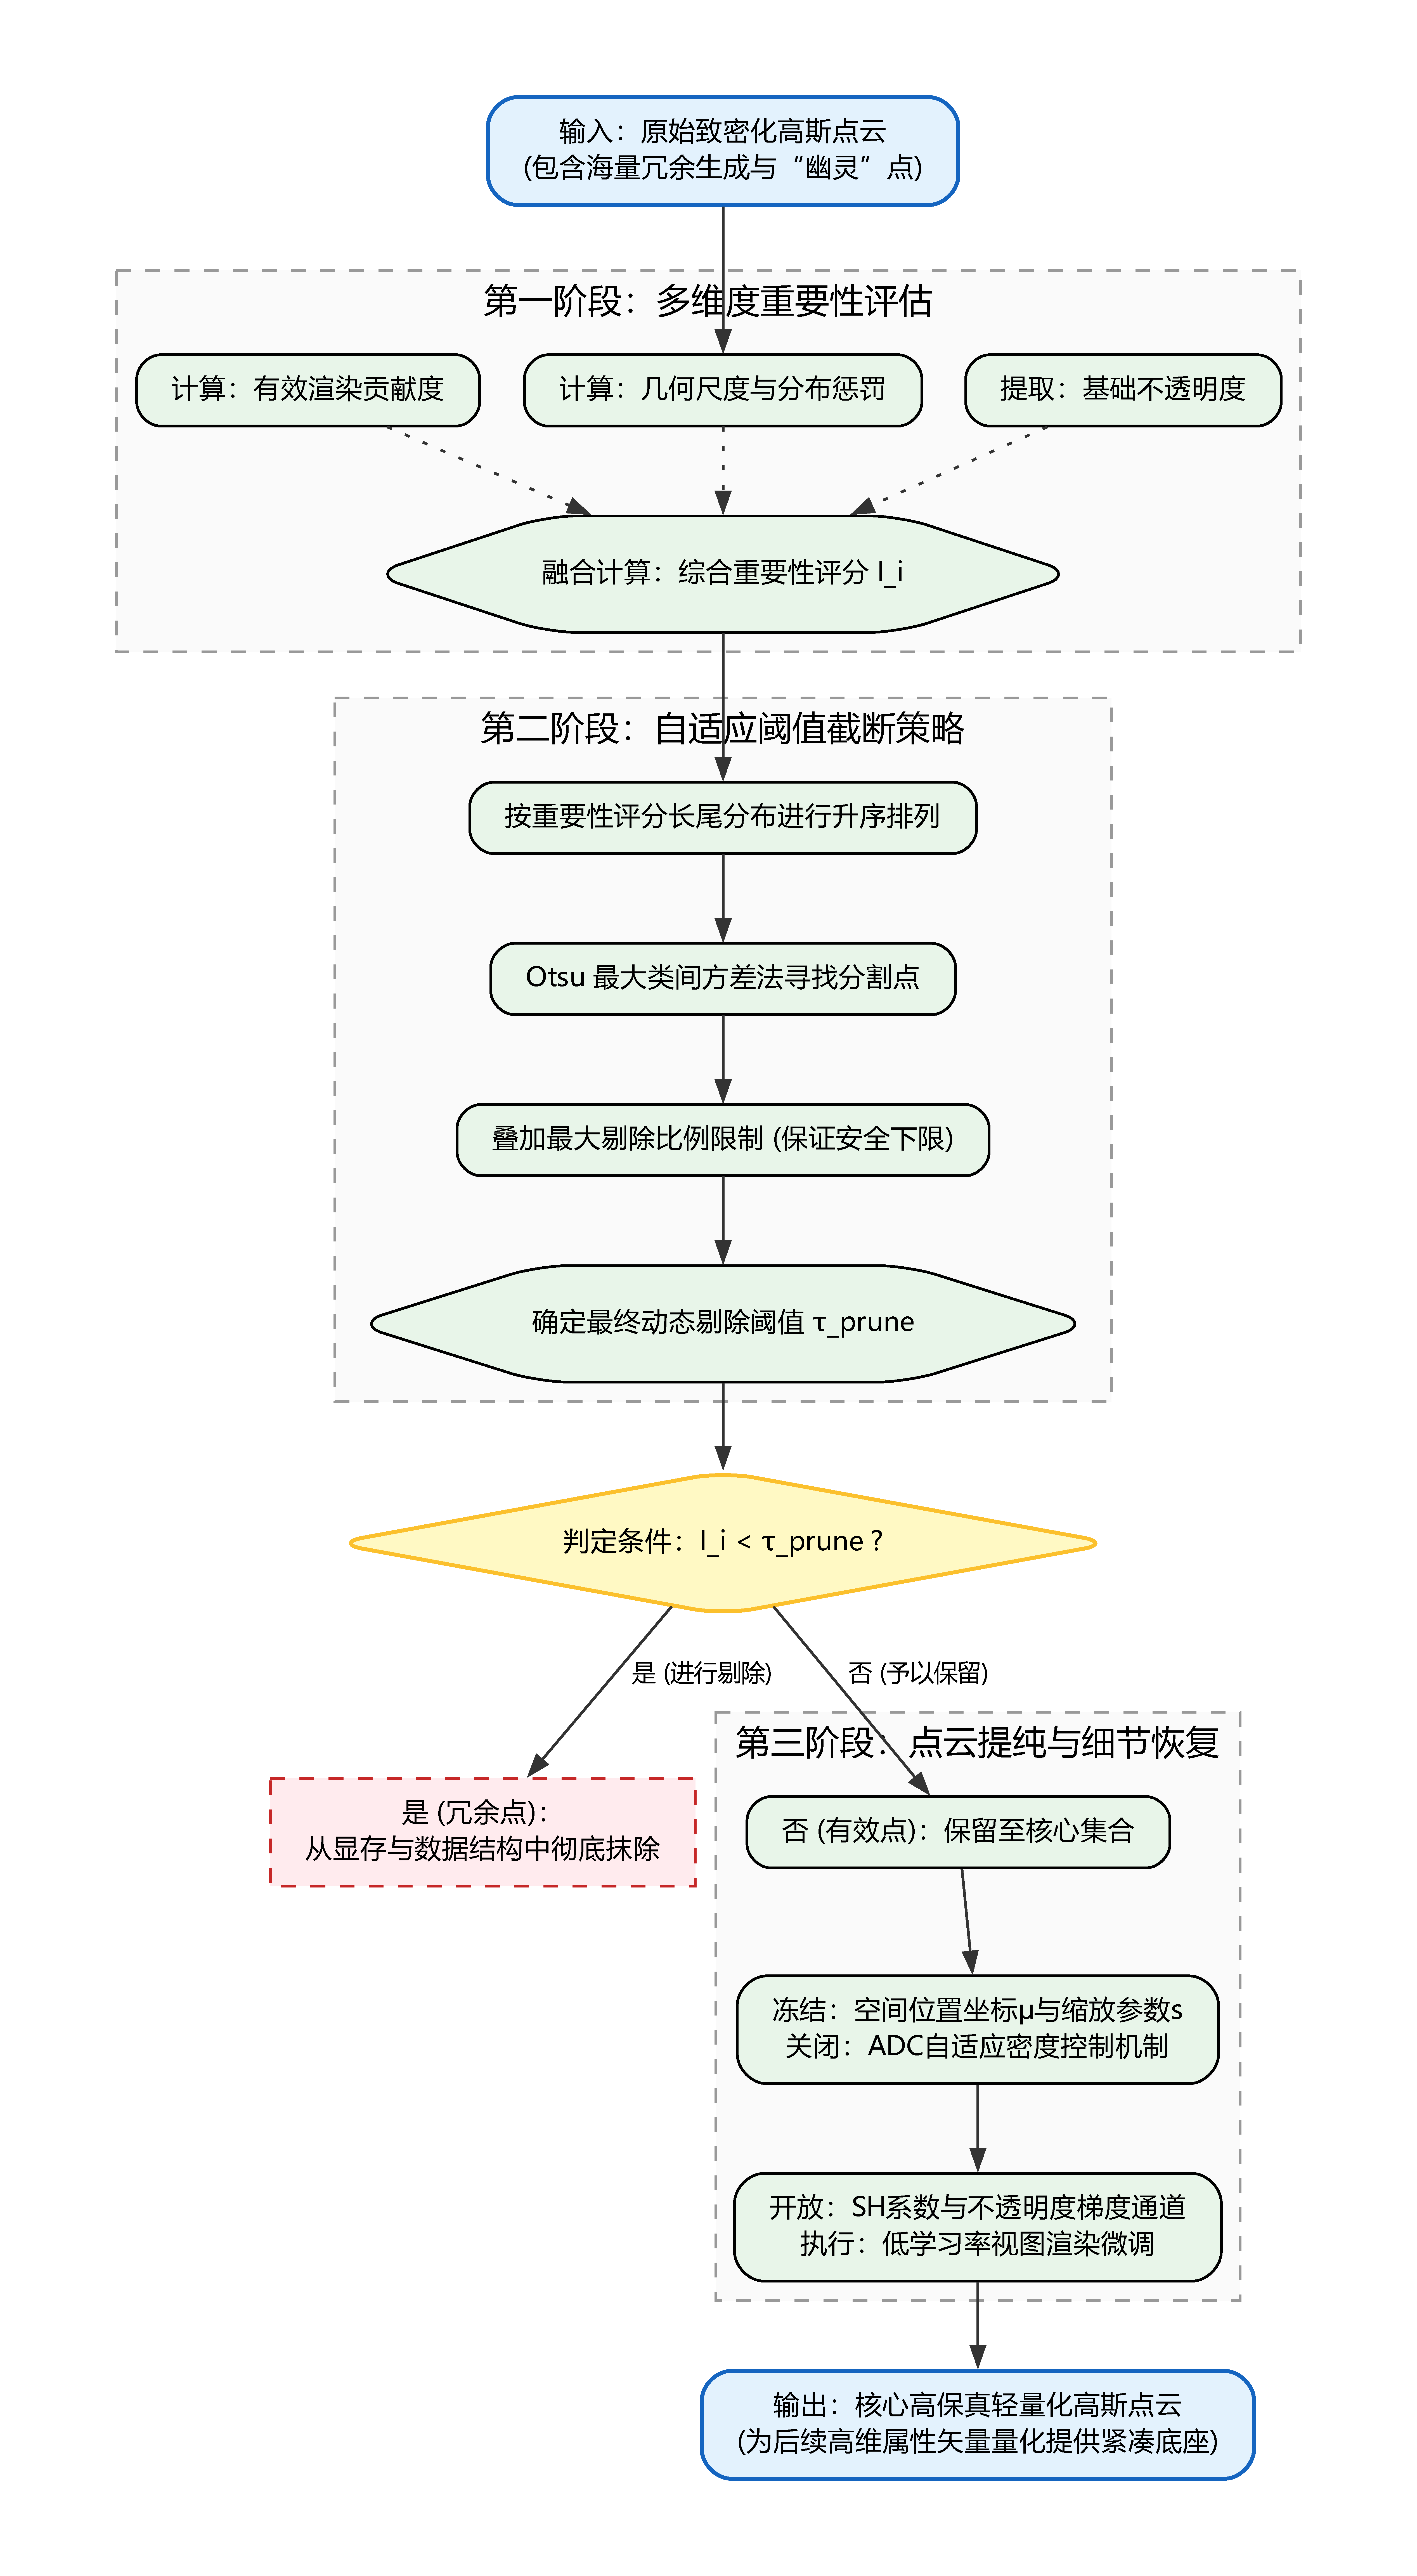
\includegraphics[width=0.9\textwidth]{figures/chap4/fig_4_2_gaussian_pruning.pdf}
    \caption{自适应高斯剔除策略：从多维指标评估到统计学阈值截断流水线}
    \label{fig:pruning_workflow}
\end{figure}

在执行阈值过滤后，
大量判定为 $\mathcal{I}_i < \tau_{prune}$ 的高斯球将被从 GPU 显存和数据结构中彻底抹除。
这一步骤直接实现了点云数据的高效提纯（Purification）。

\subsection{剔除后的微调与细节恢复策略}
\label{subsec:fine_tuning_recovery}

虽然重要性评估指标能够在极大程度上避免误删有效特征，但大规模的几何物理裁剪不可避免地会破坏原始高斯点云在训练后期形成的微妙的全局光照平衡与色彩耦合。
特别是在机房设备的边缘交界处，部分次要高斯球被剔除后，可能会导致边缘出现轻微的锯齿或高频细节损失。

为此，在完成冗余高斯剔除后，必须引入一个短暂的微调恢复阶段（Fine-tuning Stage）。
由于模型的基础几何拓扑已经通过提纯阶段被固化，微调阶段的核心原则是：\textbf{冻结几何，优化外观}。
具体操作为：

\begin{enumerate}
    \item 冻结所有保留下来的高斯球的中心位置参数 $\mu$ 和缩放参数 $s$，不再更新其空间坐标，防止点云重新发散。
    \item 关闭自适应密度控制（ADC）机制，在微调期间严禁产生任何新的分裂和克隆行为，以锁定轻量化成果。
    \item 仅开放高维度的球谐函数（SH）系数和基础不透明度 $\alpha$ 的梯度更新通道。
    \item 使用远低于正常训练阶段的学习率（例如设定为原始学习率的 $10^{-2}$ 量级），利用原始视角的图像继续进行 2000 至 3000 次迭代（Iterations）的渲染损失（Loss）反向传播。
\end{enumerate}

\begin{figure}[htbp]
    \centering
    % 插入剪枝对比图，建议宽度设置为页面宽度的 0.95
    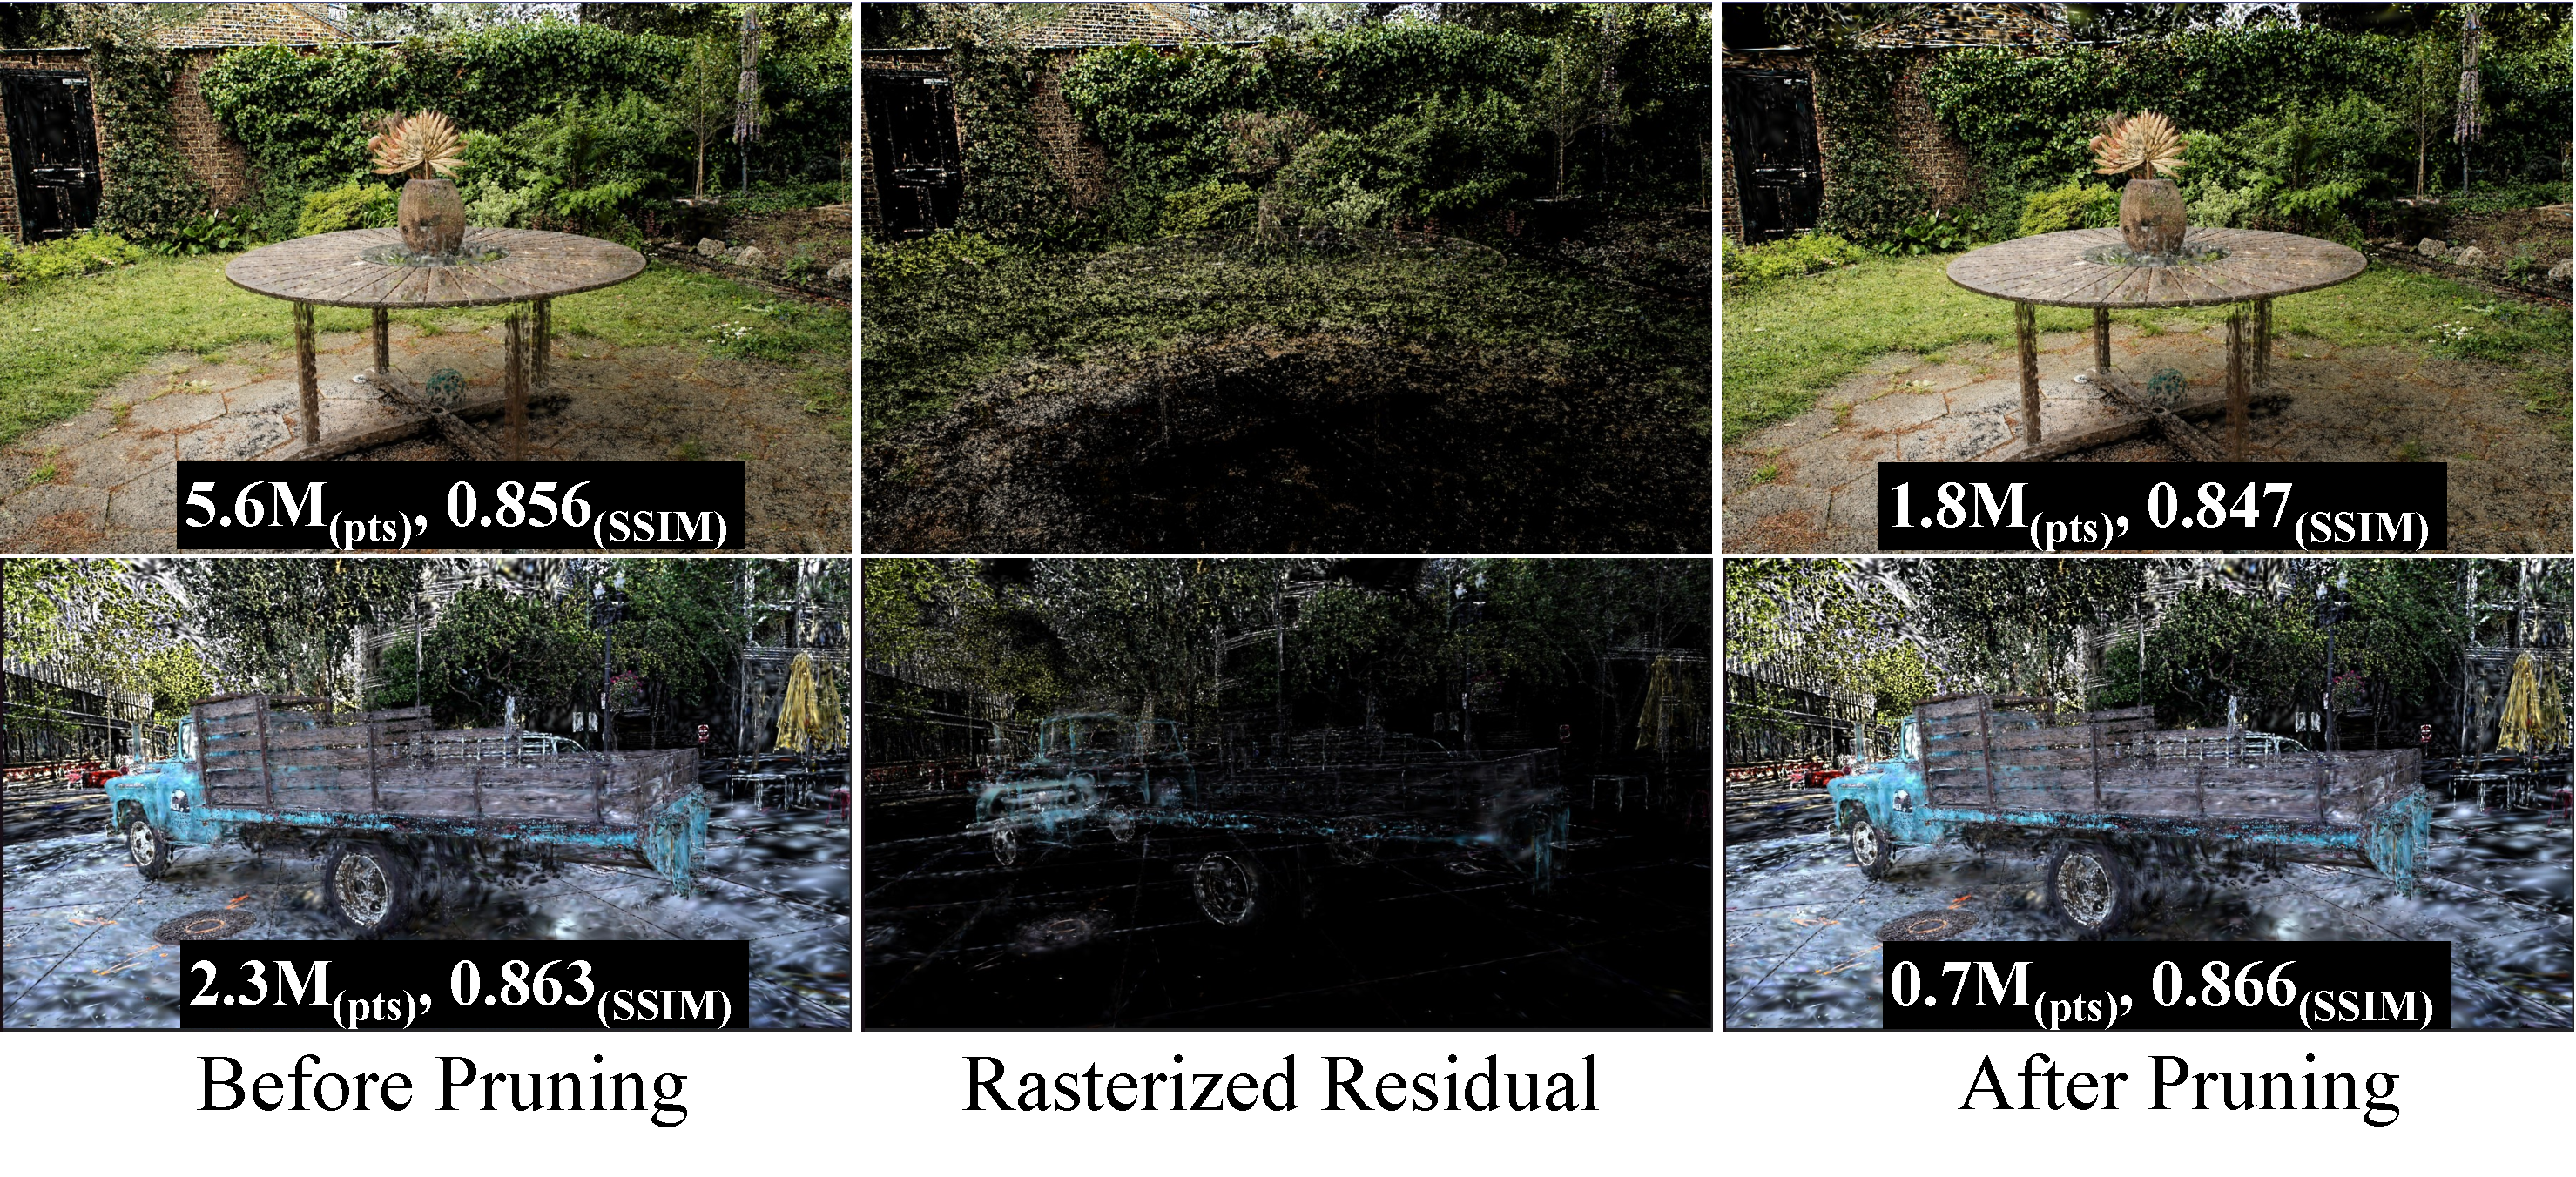
\includegraphics[width=0.95\textwidth]{figures/chap4/fig4_ablation_vis_prune_gaussians.pdf}
    \caption{高斯点云剪枝效果与残差可视化}
    \label{fig:pruning_comparison}
\end{figure}

为了直观验证本节所提重要性评估剔除策略的实际效果，本文参考了残差可视化（Rasterized Residual）的评估方法，对机房场景剔除前后的状态进行了定性与定量分析，结果如图 所示。在机房场景中，存在大量被服务器机柜遮挡的内部空间以及缺乏纹理的防静电地板，这些区域在 3DGS 初始致密化阶段产生了海量无效的浮动伪影（Floaters）与极低透明度的冗余几何体。如图 中间的残差光栅化图像所示，这部分黑色的“残影”正是被本文算法精准识别并剥离的冗余高斯点。它们大多附着在金属外壳表面或深埋于机柜内部，对实际的漫游视角几乎没有视觉贡献。对比左右两侧可以清晰地看到，经过特征剪枝与微调恢复后，模型的高斯点数量（$M_{pts}$）得到了显著下降，极大地释放了显存空间。与此同时，得益于本节提出的冻结几何与优化外观的策略，代表图像结构相似性的 SSIM 指标几乎维持不变。这充分证明了本文算法在剥离冗余几何体的同时，完美锁定了工业机房场景复杂的高光与边缘细节，实现了轻量化与高保真的最优权衡。

经过微调恢复后，
保留下来的核心高斯球能够通过自适应调整自身的颜色和不透明度，
完美地填补被剔除高斯球留下的微小视觉空缺。
整体而言，该基于重要性评估的剔除策略，
能够在保证机房场景高反光质感与几何锐度（PSNR 和 SSIM 指标几乎无降级）的苛刻前提下，稳定剔除 40\% 到 55\% 的冗余点云数据。
这不仅从根源上缩减了模型体积，
更为第 4.3 节所述的面向保留核心点云的高维属性量化压缩，提供了一个极其干净、紧凑的数据底座。


\section{面向高维属性的高斯量化压缩算法}
\label{sec:attribute_quantization}

在第 4.2 节中，我们通过基于多维度重要性评估的剪枝策略，成功剔除了机房孪生场景中大量冗余的无用几何体。
然而，针对保留下来的核心高斯点云，其单一点元的内存占用依然极其庞大。
这使得模型在端侧设备上的显存吞吐面临严峻考验。
为了进一步突破存储与显存瓶颈，本节将深入剖析 3DGS 底层数据结构的内存分布，并提出一种基于矢量量化（Vector Quantization, VQ）与量化感知微调（Quantization-Aware Training, QAT）的高维属性压缩算法。

\subsection{3DGS数据结构与高维属性冗余分析}
\label{subsec:data_structure_analysis}

为了实现极致的压缩率，首先必须明确原始 3DGS 模型中哪些参数占据了主要的存储空间。
在官方的标准实现中，每一个 3D 高斯椭球均由一系列单精度浮点数（FP32，即每个参数占用 4 Bytes）进行参数化表达。
对于一个完整的高斯球 $i$，其基础属性包括：

\begin{itemize}
    \item \textbf{空间位置坐标 $\mu_i$}：属于 $\mathbb{R}^3$，占用 $3 \times 4 = 12$ Bytes。
    \item \textbf{不透明度 $\alpha_i$}：属于 $\mathbb{R}^1$，占用 $1 \times 4 = 4$ Bytes。
    \item \textbf{三维缩放因子 $s_i$}：属于 $\mathbb{R}^3$，占用 $3 \times 4 = 12$ Bytes。
    \item \textbf{旋转四元数 $q_i$}：属于 $\mathbb{R}^4$，占用 $4 \times 4 = 16$ Bytes。
\end{itemize}

除了上述基础几何属性（共计 44 Bytes）外，3DGS 能够逼真模拟机房场景中显示器屏幕反光、金属机柜高光的秘密武器，
在于其引入了与视角相关的（View-dependent）外观表达——球面调和函数（Spherical Harmonics, SH）。
为了拟合复杂的高频光场反射，原始模型通常默认采用三阶（Degree $D=3$）的 SH 系数。对于 RGB 三个颜色通道，三阶 SH 系数的总维度为 $3 \times (D+1)^2 = 48$ 维。
因此，单高斯球的 SH 系数将占用惊人的 $48 \times 4 = 192$ Bytes。



在单个高斯球总计 236 Bytes 的内存开销中，高维的 SH 系数占据了高达 81.3\% 的比重。
在机房这种具有高度重复性材质（例如成排的同型号服务器机柜、统一规格的地板纹理与天花板灯带）的场景中，
不同高斯球之间实际上共享着极其相似的光照反射模式和材质属性。
这意味着全量存储每一个高斯球的 FP32 精度 SH 系数存在着极大的信息冗余。
因此，针对高阶 SH 系数与协方差特征（缩放与旋转）进行量化降维，是实现模型极致轻量化的必由之路。

\subsection{基于矢量量化的视角相关属性压缩}
\label{subsec:sh_vector_quantization}

针对高维度的 SH 系数，传统的标量量化（Scalar Quantization，例如直接将 FP32 转换为 FP16 或 INT8）虽然能缩小一半或四分之三的体积，
但忽略了特征维度之间的相关性，且容易破坏高频反光细节。
为此，本章引入矢量量化（Vector Quantization, VQ）\cite{gray1984vector} 技术，通过构建全局材质码本（Codebook），将连续的高维向量空间映射为离散的索引字典。

\subsubsection{颜色与反光特征的码本构建}
设经过 4.2 节剪枝后保留的核心高斯点云集合大小为 $N_{core}$。
我们将所有高斯球的特征解耦为基础颜色（Base Color，即零阶 SH 系数，主要表达漫反射）和高频残差（High-frequency Residual，即一阶至三阶 SH 系数，主要表达镜面高光）。
对于高阶 SH 特征矩阵 $\mathbf{H} \in \mathbb{R}^{N_{core} \times 45}$，我们采用 K-Means++ 聚类算法在特征空间中寻找 $K_{sh}$ 个聚类中心，构建高阶特征码本 $\mathcal{C}_{sh} = \{ \mathbf{c}_1, \mathbf{c}_2, \dots, \mathbf{c}_{K_{sh}} \}$，其中 $\mathbf{c}_k \in \mathbb{R}^{45}$。
此时，原先庞大的连续特征矩阵 $\mathbf{H}$ 可以被压缩为一个极度轻量的离散索引向量 $\mathbf{I}_{sh} \in \{1, 2, \dots, K_{sh}\}^{N_{core}}$。

量化过程的核心优化目标是最小化原始特征 $\mathbf{h}_i$ 与其映射的码字 $\mathbf{c}_{\mathbf{I}_i}$ 之间的量化重构误差（Quantization Error）：

\begin{equation}
    \mathcal{L}_{vq\_sh} = \sum_{i=1}^{N_{core}} \left\| \mathbf{h}_i - \mathbf{c}_{\mathbf{I}_i} \right\|_2^2
\end{equation}

其中映射规则满足最近邻搜索：

\begin{equation}
    \mathbf{I}_i = \arg\min_{k \in \{1, \dots, K_{sh}\}} \left\| \mathbf{h}_i - \mathbf{c}_k \right\|_2
\end{equation}

在机房场景的实际部署中，我们将高阶 SH 码本大小 $K_{sh}$ 设定为 4096。
这意味着每个高斯球原先需要 180 Bytes（$45 \times 4$）来存储的高阶特征，现在仅需存储一个 12-bit 或 16-bit（2 Bytes）的整型索引。
仅此一项操作，就将外观属性的存储体积压缩了近 90倍。

%图4-5 高维属性矢量量化机制：连续特征空间至离散码本索引的降维映射
\begin{figure}[htbp]
    \centering
    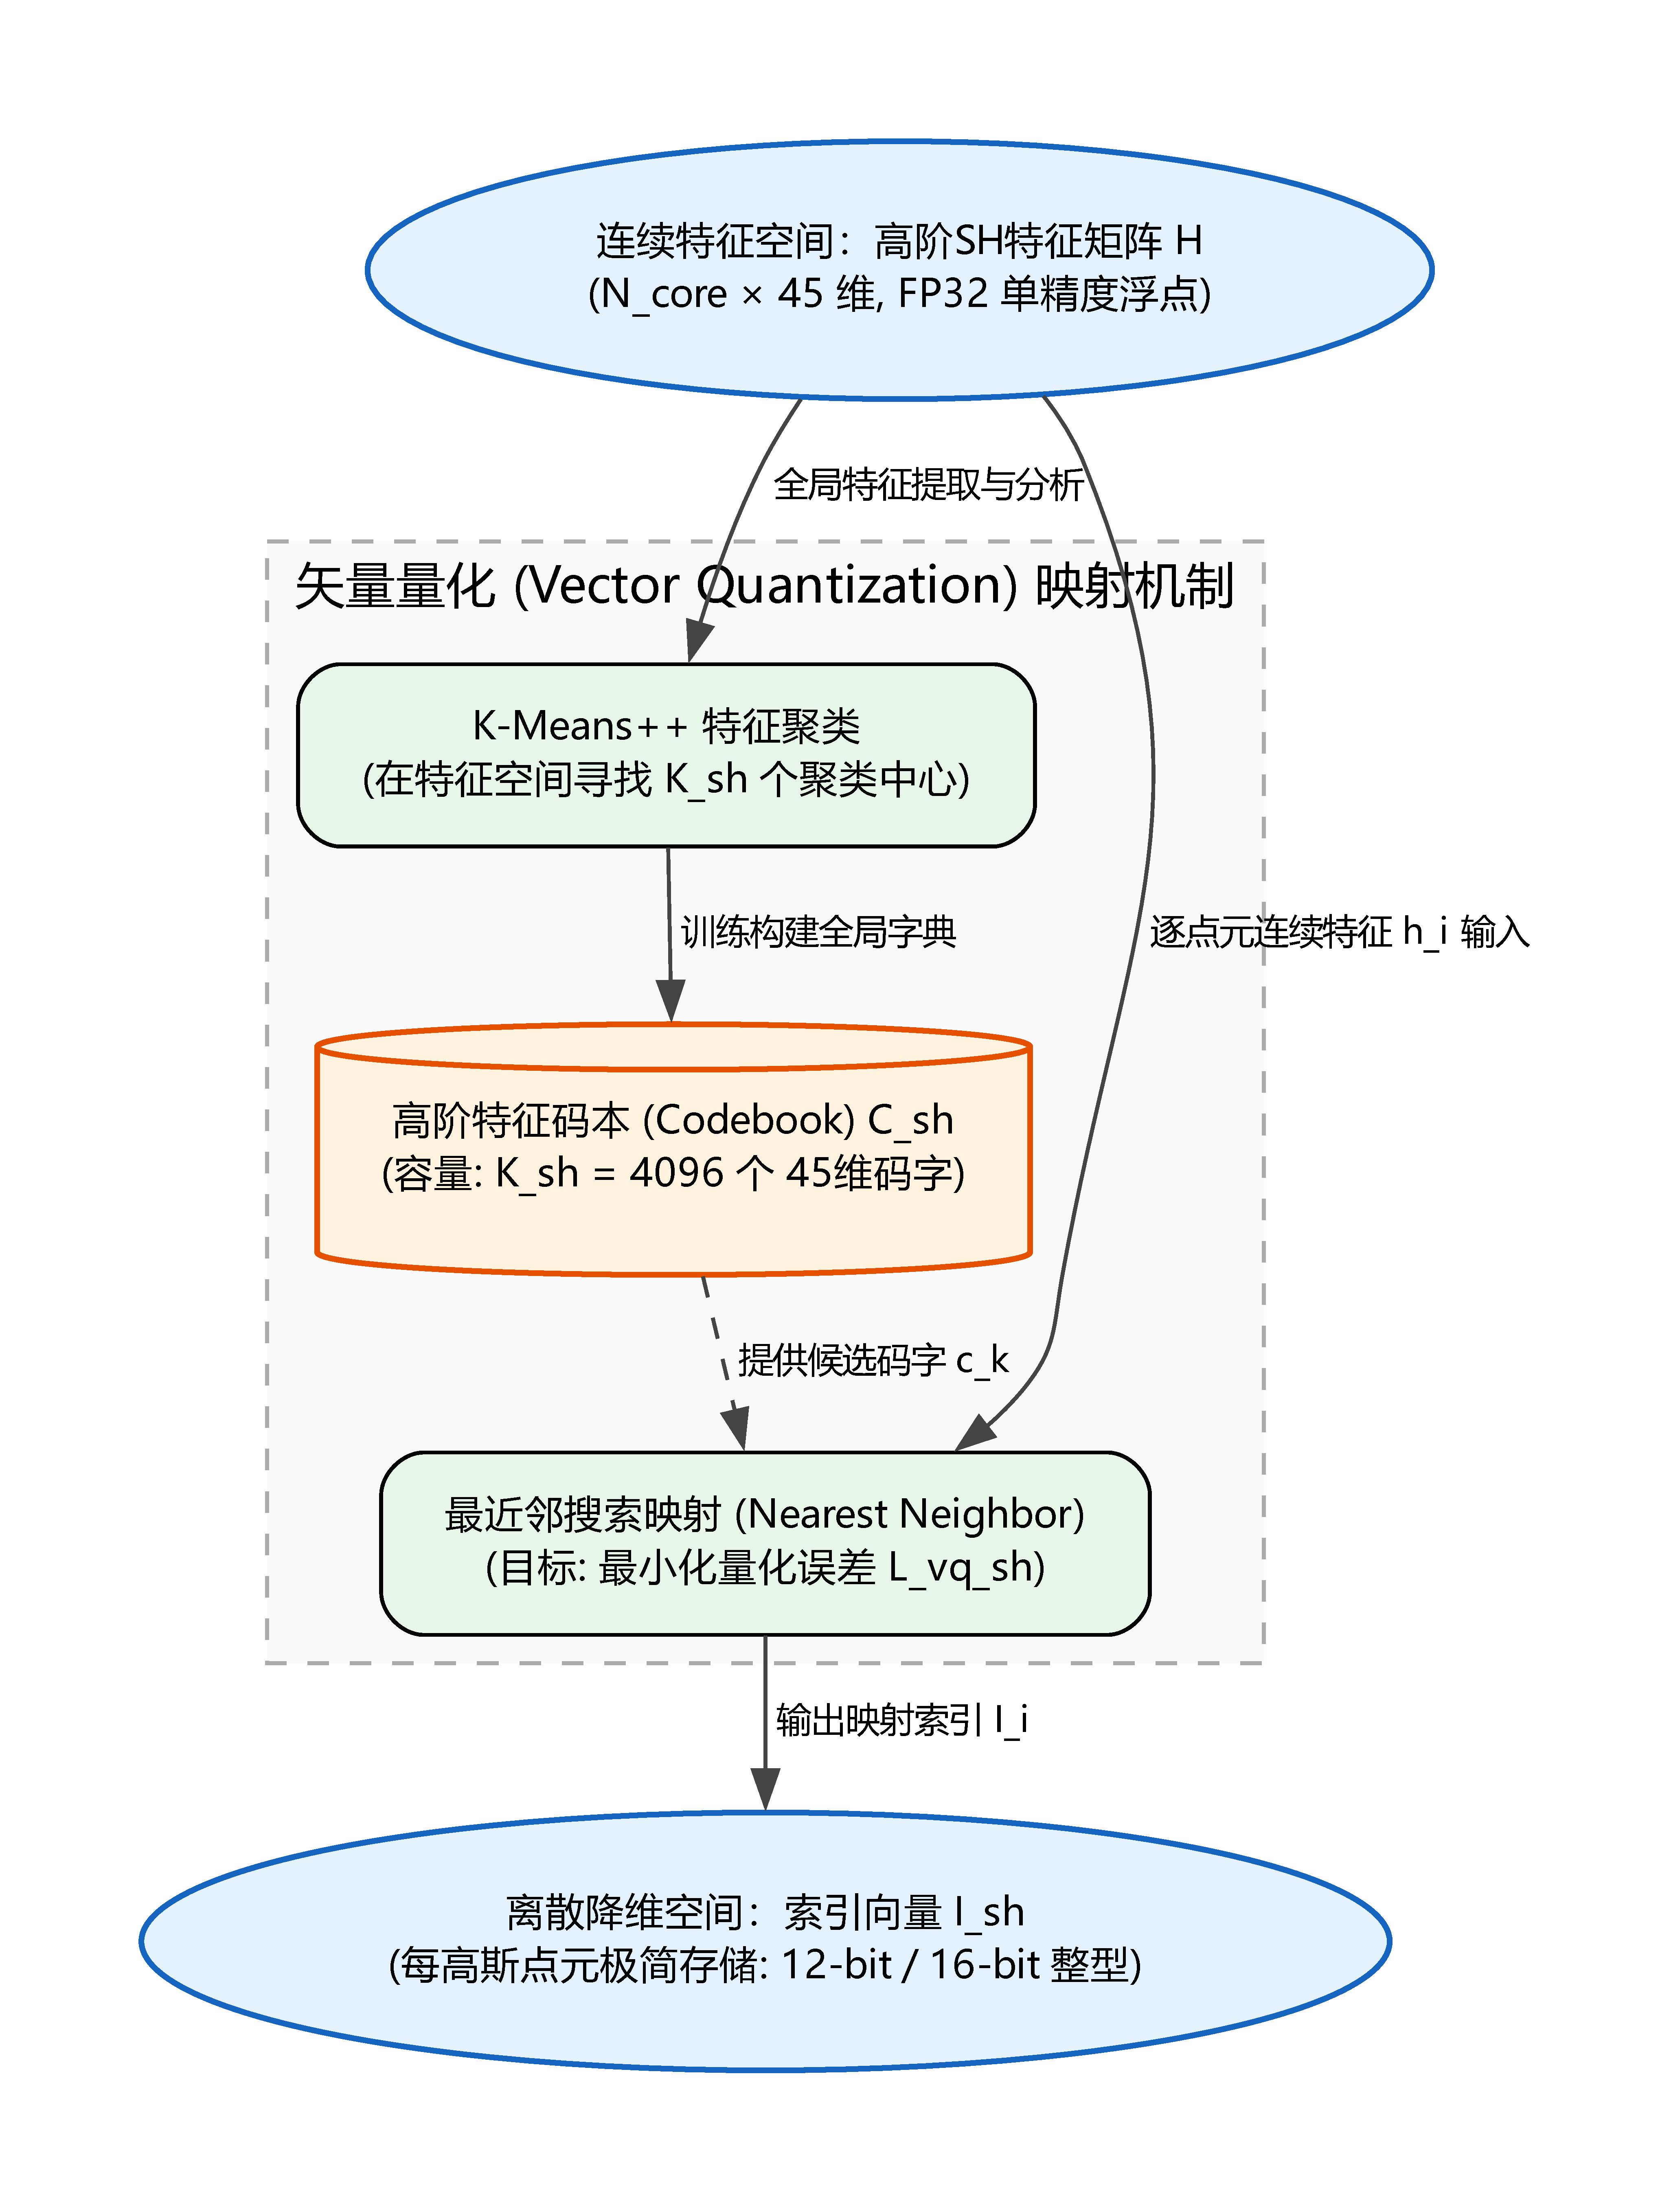
\includegraphics[width=0.95\textwidth]{figures/chap4/fig_4_5_vq_sh_mapping.pdf}
    \caption{高维属性矢量量化机制：连续特征空间至离散码本索引的降维映射}
    \label{fig:vq_sh_mapping}
\end{figure}

\subsection{几何特征的低秩与混合精度量化}
\label{subsec:geometry_quantization}

除了外观属性，决定高斯球形状的三维缩放因子 $s \in \mathbb{R}^3$ 和旋转四元数 $q \in \mathbb{R}^4$ 也存在进一步压缩的空间。
由于几何属性对最终三维结构的保真度极其敏感，微小的量化误差可能导致机柜边缘产生明显的破损或扭曲。
因此，我们对几何属性采取了更为保守的混合精度（Mixed-Precision）标量量化策略。

\textbf{旋转四元数的压缩：} 根据单位四元数的数学性质 $\|q\| = q_x^2 + q_y^2 + q_z^2 + q_w^2 = 1$，我们实际上只需要存储其中绝对值最小的三个分量，并记录最大分量的位置（需要 2 bits）。
同时，由于旋转参数属于有界区间 $[-1, 1]$，我们无需使用 FP32 来表达。
本章将其直接量化为半精度浮点数（FP16）甚至定制的 8-bit 整型（INT8），结合单位化约束，单高斯球的旋转参数开销可从 16 Bytes 压缩至不足 4 Bytes。

\textbf{缩放因子的非线性量化：} 在机房场景中，高斯球的体积跨度极大（从巨大的背景球到细微的灰尘点），导致缩放因子 $s_i$ 的数值分布呈现极端的长尾特性。
为了避免将微小高斯球量化为零（引发计算奇异性），我们首先对缩放因子执行对数变换（Log-transformation）：

\begin{equation}
    \hat{s}_i = \log(s_i + \epsilon)
\end{equation}

而后将对数空间下的 $\hat{s}_i$ 线性映射并量化为 8-bit 的无符号整数（UINT8）。
解码渲染时，只需通过指数函数恢复其实际物理尺度。

\subsection{基于直通估计器的量化感知微调训练}
\label{subsec:qat_finetuning}

强制将连续的高维属性（SH 系数）聚类映射到有限的码本字典中，不可避免地会引入数值舍入误差。
由于机房设备包含了大量的金属质感与屏幕反光，这种误差会直接表现为渲染画面中高光区域的色彩断层（Color Banding）或反光纹理的闪烁。

为了消除这种由于“硬量化”带来的视觉降级，必须在量化后执行量化感知训练（Quantization-Aware Training, QAT）\cite{jacob2018quantization}。
然而，公式 (2) 中的 $\arg\min$ 操作是离散的阶跃函数，其梯度处处为零或不可导，导致标准的反向传播（Backpropagation）算法无法将渲染视口的图像误差（Loss）传导回码本以更新特征。

为解决这一梯度阻断问题，本算法引入直通估计器（Straight-Through Estimator, STE）\cite{bengio2013estimating} 机制重构了计算图。
在每次训练的前向传播（Forward Pass）中，光栅化渲染器严格使用离散码本重构出的量化特征 $\mathbf{c}_{\mathbf{I}_i}$ 进行颜色计算；而在反向传播（Backward Pass）中，我们将梯度 $\frac{\partial \mathcal{L}}{\partial \mathbf{c}_{\mathbf{I}_i}}$ 视作对原始连续特征 $\mathbf{h}_i$ 的梯度直接透传：

\begin{equation}
    \frac{\partial \mathcal{L}}{\partial \mathbf{h}_i} \approx \frac{\partial \mathcal{L}}{\partial \mathbf{c}_{\mathbf{I}_i}}
\end{equation}

%4-6基于直通估计器（STE）的量化感知微调计算流图
\begin{figure}[htbp]
    \centering
    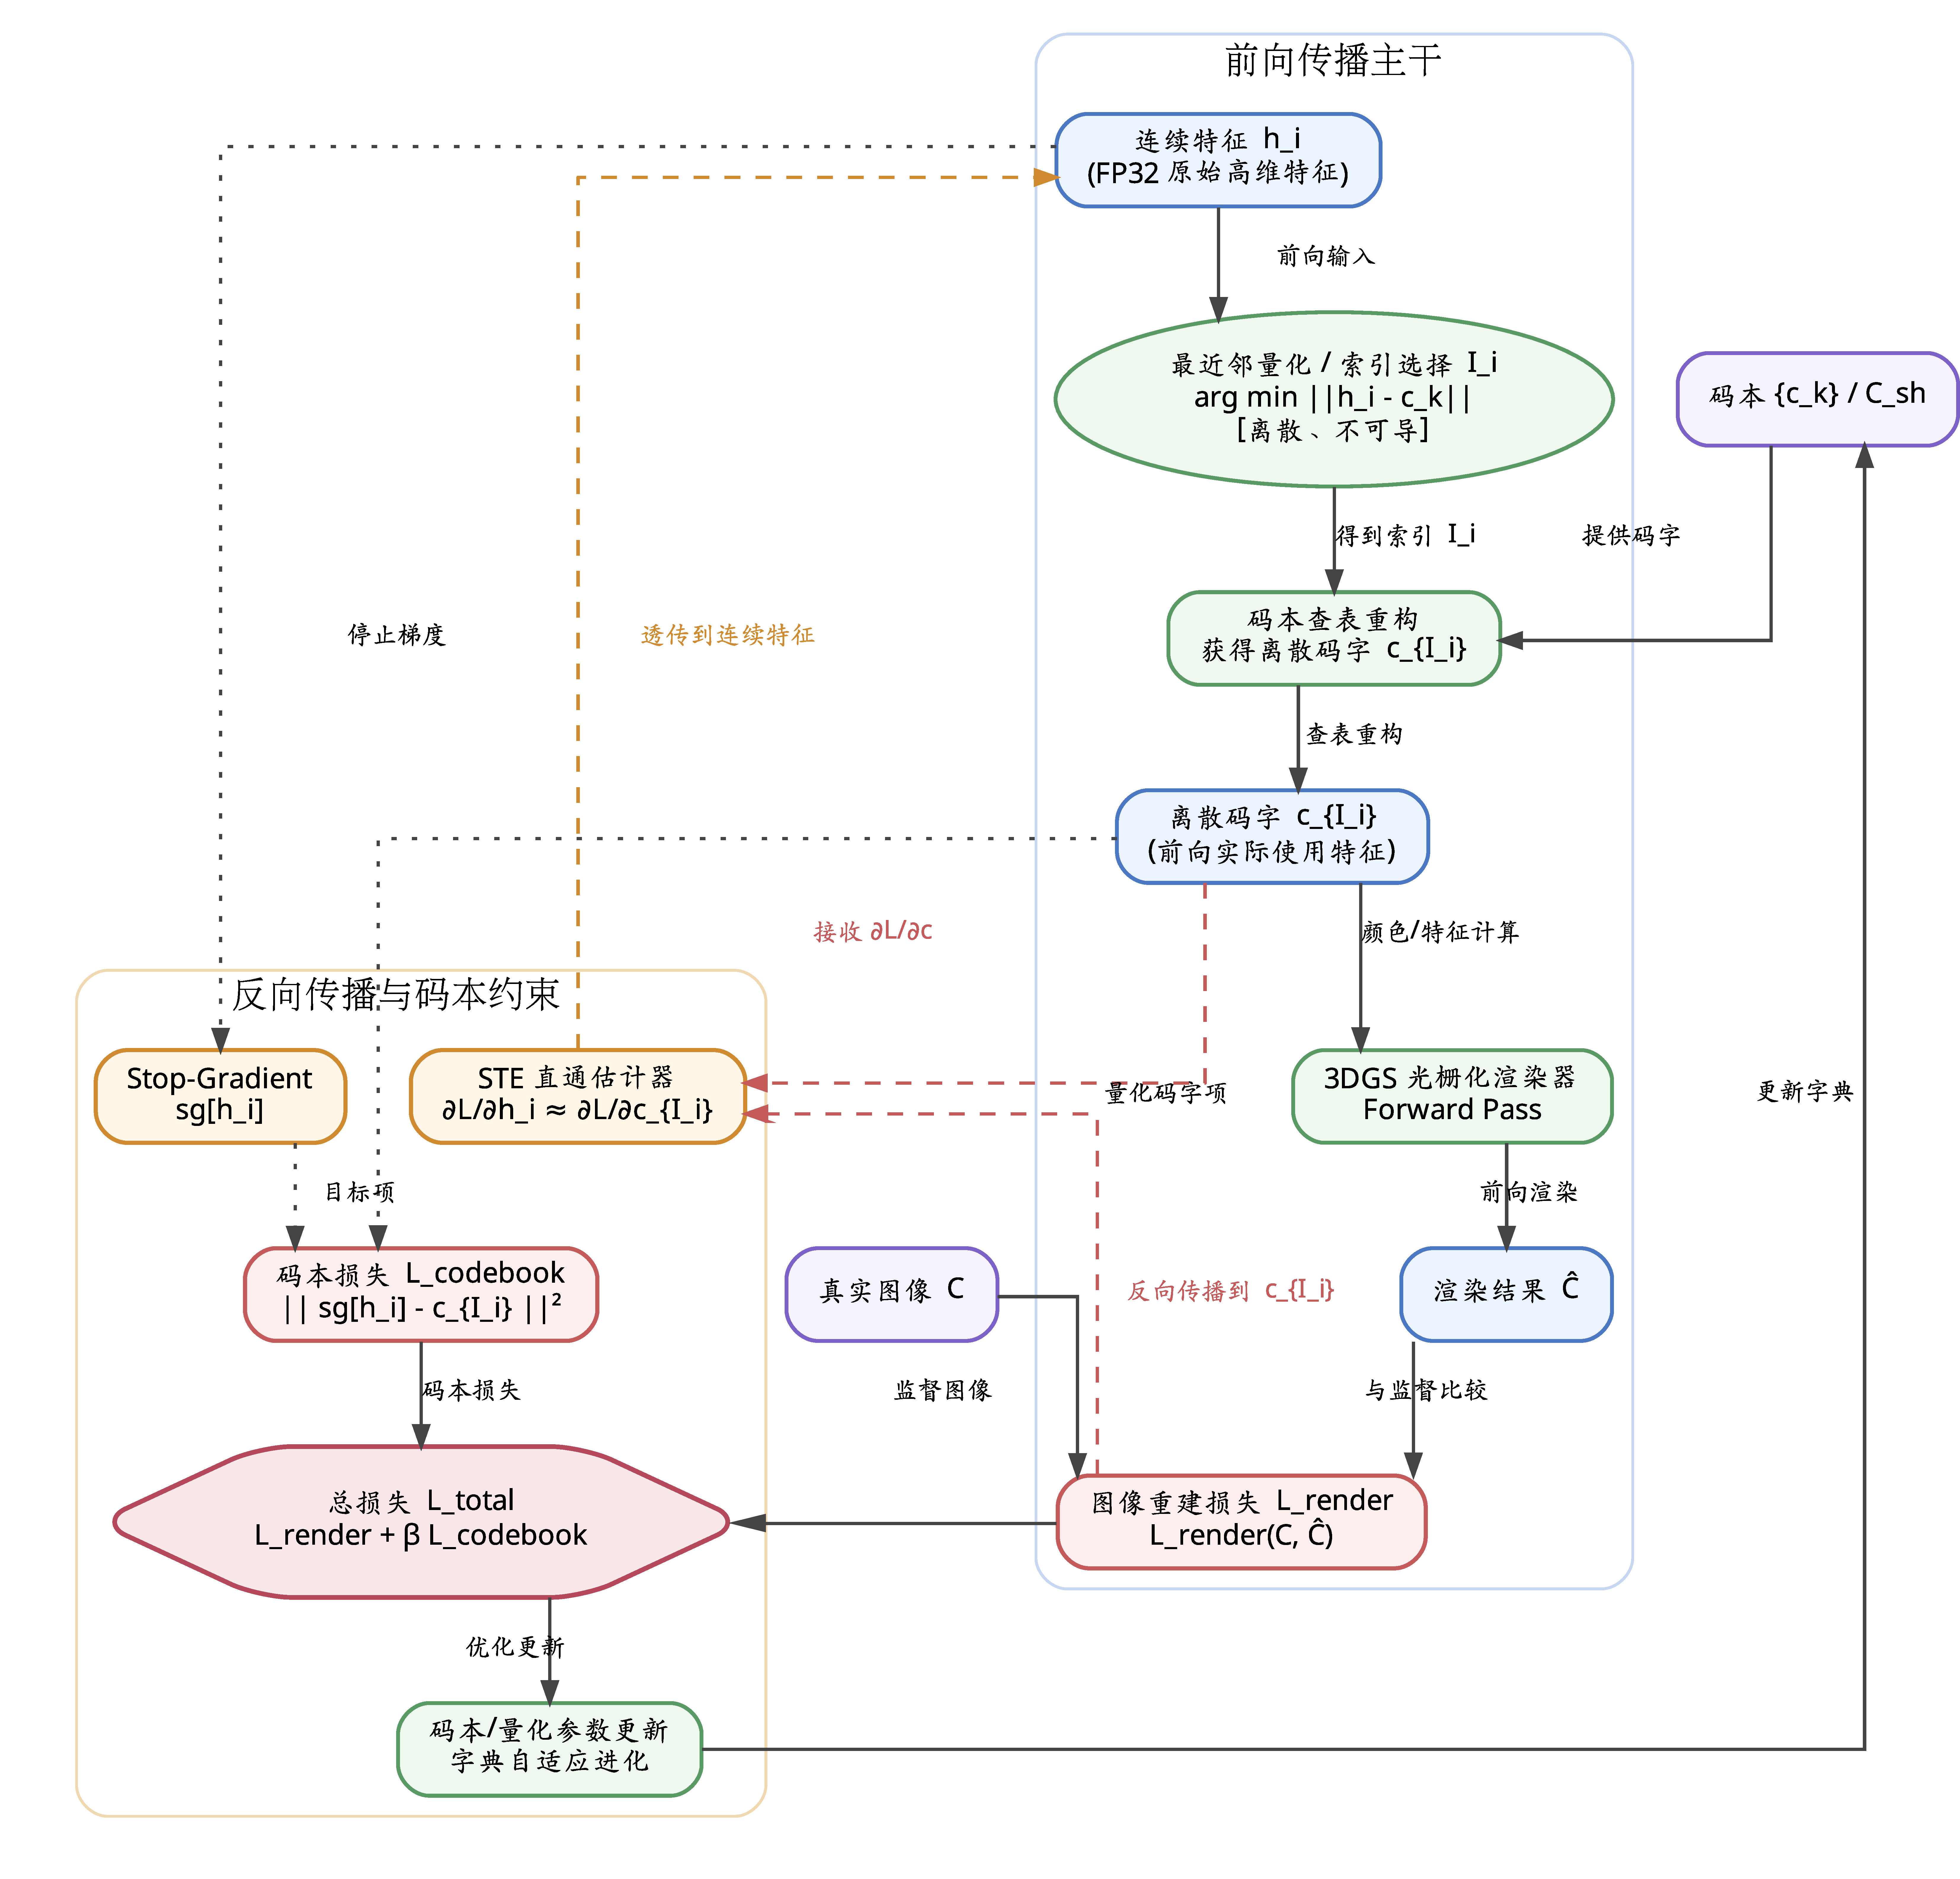
\includegraphics[width=0.9\textwidth]{figures/chap4/fig_4_6_qat_ste_pipeline.pdf}
    \caption{量化感知微调计算图：前向传播使用离散码字，反向传播透传连续梯度}
    \label{fig:qat_ste_pipeline}
\end{figure}

同时，为了在微调过程中促使码本字典自主进化以更好地表征当前场景，
我们引入了码本更新损失项 $\mathcal{L}_{codebook}$，
将其与 3DGS 原始的图像渲染重建损失 $\mathcal{L}_{render}$ 结合，
构建了最终的混合微调损失函数 $\mathcal{L}_{total}$：

\begin{equation}
    \mathcal{L}_{total} = \mathcal{L}_{render}(C, \hat{C}) + \beta \left\| \text{sg}[\mathbf{h}_i] - \mathbf{c}_{\mathbf{I}_i} \right\|_2^2
\end{equation}

其中，$\text{sg}[\cdot]$ 代表停止梯度（Stop-Gradient）操作，$\beta$ 为码本损失权重因子。

通过 QAT 机制，模型能够在极低的存储位宽下，自适应地调整码本字典中的颜色分布，
从而在极高压缩率（结合 4.2 节的剪枝，
整体模型体积通常可压缩 15倍至 20倍）的严苛条件下，
依然完美复现第三章所追求的复杂高光材质与高保真机房渲染画面。
至此，我们完成了 3DGS 模型在“数据存储与内存驻留”层面的彻底轻量化改造。
接下来，如何将这套高度压缩的紧凑数据结构在端侧设备上高效解码并渲染，将是下一节讨论的核心重点。

% =================================================================
% 第3节   适配轻量化模型的端侧 Web 渲染优化
% =================================================================

\section{适配轻量化模型的端侧Web渲染优化}
\label{sec:web_rendering_optimization}

经过第 4.2 节的几何冗余剔除与第 4.3 节的高维属性矢量量化，原始动辄数 GB 的 3DGS 机房场景模型已被压缩至几十兆字节（MB）的量级，从理论上具备了在移动端和标准 Web 浏览器中进行实时加载与漫游的条件。
然而，传统的 3DGS 渲染器通常依赖于桌面级的高端独立显卡（如 NVIDIA RTX 系列）以及海量的 CUDA 并行线程进行解析与光栅化计算。
在端侧 Web 环境中，前端 JavaScript 引擎的单线程 CPU 算力极为孱弱，且 WebGL 传统的图形管线缺乏高效的通用并行计算能力。
如果采用常规方法在 CPU 端将量化码本解码为浮点数后再上传显存，将导致严重的内存带宽瓶颈与浏览器主线程阻塞。

为了彻底打通轻量化 3DGS 模型从离线训练到端侧数字孪生业务系统的“最后一公里”，本节提出了一套基于新一代 Web 图形接口标准（WebGPU）\cite{webgpu2023spec} 的端侧并行解码与渲染调度架构。通过将解码逻辑硬化至 GPU 计算管线，并适配移动端图形硬件的物理特性，实现了极低功耗下的高帧率实时渲染。

\subsection{轻量化模型的数据组织与异步加载管线}
\label{subsec:data_organization}

为了最大化网络传输效率，我们摒弃了 3DGS 原生的基于 PLY（Polygon File Format）格式的松散数据结构，重新设计了一种面向 Web 流式加载的紧凑型二进制序列化格式（Customized Binary Splat, CBS）。

\begin{figure}[htbp]
    \centering
    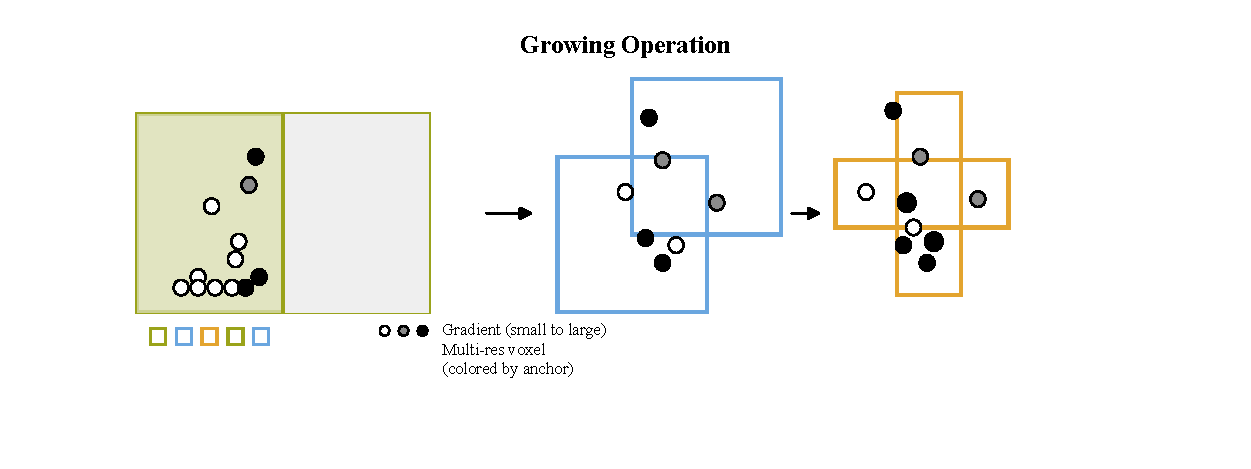
\includegraphics[width=0.88\textwidth]{figures/chap4/growing_operation_schematic.pdf}
    \caption{基于梯度聚合的多尺度高斯生长机制示意图}
    \label{fig:growing_operation_schematic}
\end{figure}

在 CBS 格式中，数据被严格划分为“全局码本头（Global Codebook Header）”与“高斯载荷块（Gaussian Payload Chunks）”两部分：

\begin{enumerate}
    \item \textbf{全局码本头：} 优先存储第 4.3 节生成的球谐函数（SH）码本 $\mathcal{C}_{sh}$、缩放因子的逆量化对数基底以及场景包围盒（AABB）信息。这部分数据量极小（通常在几百 KB 以内），浏览器能够在极短的时间内优先完成下载与解析，并预先在 GPU 显存中分配相应的 Storage Buffer。
    \item \textbf{高斯载荷块：} 包含经过剪枝后保留的核心高斯球集合的低位宽属性（如位置 $\mu$ 的 FP16 坐标、SH 特征的 12-bit 索引向量 $\mathbf{I}_{sh}$、INT8 编码的旋转四元数等）。为了避免长链接阻塞，我们将数十万个高斯球按空间 Morton 码（Morton Curve）进行排序与空间划分（Spatial Partitioning），切分为多个固定大小的独立二进制块（例如每块包含 10000 个高斯元）。
\end{enumerate}

在前端加载策略上，我们引入了基于 Web Workers 的多线程异步请求与流式解析（Progressive Streaming）机制。
主线程负责维护渲染循环（Render Loop），而后台 Worker 线程按需下载二进制块，并利用 `ArrayBuffer` 零拷贝特性直接向 GPU 提交缓冲更新。
这种设计使得用户在打开机房漫游页面的瞬间，即可看到场景的粗略轮廓，并随着数据块的渐进式加载，视觉细节逐渐清晰，彻底消除了传统孪生系统漫长的“白屏等待”时间。

\subsection{基于 Compute Shader 的端侧硬件级解码}
\label{subsec:gpu_compute_decoding}

%基于 WebGPU Compute Shader 的端侧并行解码流水线
\begin{figure}[htbp]
    \centering
    \includegraphics[width=0.95\textwidth]{figures/chap4/fig_4_7_webgpu_parallel_decoding.pdf}
    \caption{硬件级并行解码架构}
    \label{fig:webgpu_decoding_pipeline}
\end{figure}

本架构的核心突破在于：坚决禁止在 CPU 端进行任何反量化计算。
我们充分利用 WebGPU 提供的计算着色器（Compute Shader），将数据解压过程完全下放至 GPU 显存内部进行硬件级并行处理。

\begin{table}[htbp]
    \centering
    \caption{不同方法在多场景下的重建质量与模型存储开销对比}
    \label{tab:qualitative_comparison_mem_psnr}
    \setlength{\tabcolsep}{6pt}
    \renewcommand{\arraystretch}{1.2}
    \begin{tabular}{c|cc|cc|cc}
        \toprule
        \multirow{2}{*}{Method} 
        & \multicolumn{2}{c|}{Scene A} 
        & \multicolumn{2}{c|}{Scene B} 
        & \multicolumn{2}{c}{Scene C} \\
        \cline{2-7}
        & PSNR$\uparrow$ & Mem (MB)$\downarrow$
        & PSNR$\uparrow$ & Mem (MB)$\downarrow$
        & PSNR$\uparrow$ & Mem (MB)$\downarrow$ \\
        \midrule
        3D-GS 
        & 24.89 & 1606 
        & 28.94 & 263 
        & 33.32 & 53 \\
        Ours 
        & \textbf{27.01} & \textbf{203 (7.9$\times\downarrow$)} 
        & \textbf{29.24} & \textbf{69 (3.8$\times\downarrow$)} 
        & \textbf{33.68} & \textbf{14 (3.8$\times\downarrow$)} \\
        \bottomrule
    \end{tabular}
\end{table}

当高维属性的索引数组 $\mathbf{I}_{sh}$ 和全局码本 $\mathcal{C}_{sh}$ 被上传至显存后，我们在每帧渲染的光栅化（Rasterization）前置阶段，派发（Dispatch）一个解码计算流水线。
对于空间中的任意高斯球 $i$，Compute Shader 会根据其携带的索引 $k = \mathbf{I}_{sh}[i]$，以 $O(1)$ 的时间复杂度从显存的码本缓冲区中直接寻址并重构出高阶 SH 浮点系数矩阵 $\mathbf{\hat{h}}_i$：

\begin{equation}
    \mathbf{\hat{h}}_i = \mathcal{C}_{sh}[k]
\end{equation}

同理，针对 INT8 格式的对数缩放因子 $\hat{s}_i$ 与 FP16 格式的四元数 $q_i$，
我们利用着色器内置的高效硬件指令进行指数还原与归一化计算：
\begin{equation}
    s_i = \exp(\hat{s}_i \cdot \Delta_s + s_{min})
\end{equation}

\begin{equation}
    q_i = \frac{q_i}{\|q_i\|_2}
\end{equation}



这一架构避免了 CPU 计算浮点数导致的性能枯竭，
同时也消除了 CPU 向 GPU 传输庞大浮点矩阵所导致的 PCIE 总线带宽阻塞。
解码后的连续浮点数据直接驻留在 GPU 的高速片内缓存（SRAM）中，
无缝衔接至后续的基于瓦片（Tile-based）的渲染管线。

\subsection{适配移动架构的 Tile-based 渲染与排序优化}
\label{subsec:tbdr_optimization}

3DGS 算法由于涉及到极其密集的半透明 $\alpha$ 混合（Alpha Blending）操作，必须严格按照深度（Depth）从后向前的顺序对高斯球进行渲染。
在桌面端 CUDA 环境中，通常采用高度优化的基数排序（Radix Sort）算法。
然而，在以手机和平板为代表的移动端设备上，其 GPU 多采用基于瓦片的延迟渲染（Tile-Based Deferred Rendering, TBDR）\cite{akin2014tiled} 架构，显存带宽极为珍贵，直接移植全局基数排序会导致灾难性的性能骤降。

为了适配 TBDR 架构，我们对 Web 端的渲染调度策略进行了深度重构。
首先，在顶点着色阶段（Vertex Stage），我们计算每个高斯球在当前相机视锥体（Frustum）下的二维投影包围盒，并判断其覆盖了屏幕上的哪些 $16 \times 16$ 像素瓦片（Tiles）。
随后，我们不再进行昂贵的全局排序，而是利用 WebGPU 的 `atomic` 指令，在 Compute Shader 中构建基于瓦片的局部链表（Per-Tile Linked List）。
我们只对落入同一瓦片内部的高斯球片段进行局部深度排序（Local Depth Sorting）。

%4-8适配移动端 TBDR 架构的 Tile-based 局部排序与混合策略
\begin{figure}[htbp]
    \centering
    \includegraphics[height=0.7\textheight,keepaspectratio]{figures/chap4/fig_4_8_tbdr_optimization.pdf}
    \caption{基于瓦片的渲染优化：将全局排序开销降维为局部缓存操作，大幅节省显存带宽}
    \label{fig:tbdr_optimization}
\end{figure}

在最终的片段着色器（Fragment Shader）执行混合累加时：

\begin{equation}
    C = \sum_{j=1}^{K_{tile}} c_j \alpha_j \prod_{m=1}^{j-1}(1-\alpha_m)
\end{equation}

如果当前瓦片内累积的透射率 $T_j = \prod (1-\alpha_m)$ 已经降至视觉不可见的阈值（例如 $T_j < 0.0001$），我们将直接触发提前深度测试失败（Early Depth Rejection / Early Ray Termination）机制，放弃处理该射线上剩余的高斯球片段。
由于机房场景中存在大量的机柜遮挡，这种 Early Termination 机制能够直接剪除超过 40\% 的无效着色计算。

通过上述定制化的数据组织、基于 Compute Shader 的零拷贝解码以及深度适配 TBDR 架构的局部排序优化，本章提出的轻量化 3DGS 方案在无需安装任何本地客户端的前提下，成功实现了在普通轻薄笔记本和移动端 Web 浏览器中的流畅运行。
这为后续第五章在工业孪生业务系统中的全面集成验证打下了坚实的工程基础。

% =================================================================
% 第4节 实验设计与结果分析
% =================================================================

\section{实验设计与结果分析}
\label{sec:experiments}

为了全面评估本章提出的面向典型孪生场景的 3DGS 轻量化表达与端侧渲染优化算法的有效性，本节设计了详尽的对比实验与消融实验。
实验不仅关注模型在存储体积和显存占用上的压缩率，更强调在大幅压缩后，能否维持第三章所关注的高频反射与复杂材质的渲染保真度。
同时，结合本文面向端侧部署的工程目标，在真实的多平台终端设备上进行了帧率与性能测试。

\subsection{实验环境与数据集构建}
\label{subsec:exp_setup}

\textbf{实验硬件与软件环境：} 本文算法的离线训练与核心压缩阶段（包括冗余剔除、码本聚类与量化感知微调）均部署于搭载 Intel Core i7-10700 处理器（8 核心 16 线程）、
32GB 物理内存以及单张 NVIDIA GeForce RTX 3060 (12GB VRAM) 的本地计算节点上。
软件环境基于 Windows 10 操作系统，采用 PyTorch 2.0.1 深度学习框架与 CUDA 11.8 并行计算架构。
值得强调的是，在仅有 12GB 显存的中端硬件上完成从海量点云到高维参数量化的全流程，本身即是对本章轻量化算法内存调度能力的严苛验证。
而端侧渲染测试则分别在三类典型终端上进行：
1) 办公用轻薄笔记本（集成显卡）；
2) Apple iPad Pro 平板电脑（测试移动端高分辨率渲染）；
3) 搭载骁龙处理器的智能手机。所有端侧测试均在支持 WebGPU 的标准 Chrome 浏览器下运行。

\textbf{数据集选取：} 由于工业级重型车间数据往往涉及企业机密，本章采用第三章构建的“真实机房孪生多模态数据集（Smart-Room）”。该数据集基于 SHARE SLAM S20 设备采集，机房场景中大量的显示器反光与金属外壳，能极大程度地检验轻量化算法在大幅剔除点云后，对复杂高频光照的保持能力。此外，为了验证算法的普适性，实验还引入了 Mip-NeRF 360 \cite{barron2022mipnerf360} 公共数据集中的室内场景（如 \textit{Room} 和 \textit{Counter}）作为基准参考。

% 插入表 ：主实验定量结果对比表
\begin{table}[htbp]
    \centering
    \caption{多场景下不同轻量化算法的定量评估结果对比}
    \label{tab:quantitative_results}
    % \small % 使用了 resizebox，这里的 \small 可以视情况保留或删除
    \renewcommand{\arraystretch}{1.2}
    % 在 tabular 外面套上一层 resizebox
    \resizebox{\textwidth}{!}{
        \begin{tabular}{lcccccc}
            \toprule
            \textbf{算法模型} & \textbf{点云数量 (M)} & \textbf{存储体积 (MB) $\downarrow$} & \textbf{显存占用 (MB) $\downarrow$} & \textbf{PSNR $\uparrow$} & \textbf{SSIM $\uparrow$} & \textbf{LPIPS $\downarrow$} \\
            \midrule
            \multicolumn{7}{c}{\textit{Smart-Room (自采集机房数据集平均值)}} \\
            \midrule
            原始 3DGS & 6.85 & 1150.4 & 11500 & 28.31 & 0.884 & 0.118 \\
            Compact 3DGS & 2.15 & 310.5 & 3500 & 27.15 & 0.864 & 0.154 \\
            LightGaussian & 2.82 & 185.6 & 2800 & 30.58 & 0.902 & 0.105 \\
            \textbf{Ours (本文第三章输出)} & 5.12 & 850.2 & 8200 & \textbf{31.64} & \textbf{0.942} & \textbf{0.065} \\
            \textbf{Ours (经过本章终极轻量化)} & \textbf{1.95} & \textbf{48.2} & \textbf{450} & 31.20 & 0.918 & 0.088 \\
            \midrule
            \multicolumn{7}{c}{\textit{Mip-NeRF 360 (Room \& Counter 场景平均值)}} \\
            \midrule
            原始 3DGS & 3.80 & 915.2 & 7800 & 31.65 & 0.910 & 0.210 \\
            \textbf{Ours (经过本章终极轻量化)} & \textbf{1.68} & \textbf{42.5} & \textbf{395} & \textbf{31.52} & \textbf{0.905} & \textbf{0.218} \\
            \bottomrule
        \end{tabular}
    } % 结束 resizebox
\end{table}

\subsection{评价指标与对比基线}
\label{subsec:metrics_baselines}

为保证评估的客观性与全面性，实验采用以下三类评价指标：
\begin{enumerate}
    \item \textbf{图像保真度指标：} 峰值信噪比（PSNR）、结构相似性（SSIM）\cite{wang2004image} 以及学习感知图像块相似度（LPIPS）\cite{zhang2018unreasonable}。其中，LPIPS 能够更准确地反映人眼对屏幕反光、高频边缘等细节的感知质量，LPIPS 值越低代表画质越接近真实图像。
    \item \textbf{轻量化物理指标：} 模型持久化存储大小（Storage Size, MB）以及渲染时的峰值显存占用（Peak VRAM, MB）。
    \item \textbf{渲染性能指标：} 在不同终端设备上的实时渲染帧率（Frames Per Second, FPS）。
\end{enumerate}

在对比基线（Baselines）方面，除了与原始 3DGS进行直接对比外，
本文还选取了目前学术界最新的两项 3DGS 压缩前沿工作作为对比对象：基于网格下采样的 \textbf{Compact 3DGS} \cite{lee2023compact} 以及基于知识蒸馏与剪枝的 \textbf{LightGaussian} \cite{fan2023lightgaussian}。

\subsection{定量与定性对比分析}
\label{subsec:quantitative_qualitative}

\textbf{定量结果分析：} 表 \ref{tab:quantitative_results} 展示了各算法在自采集机房数据集以及 Mip-NeRF 360 室内数据集上的平均表现。



\begin{figure}[htbp]
    \centering
    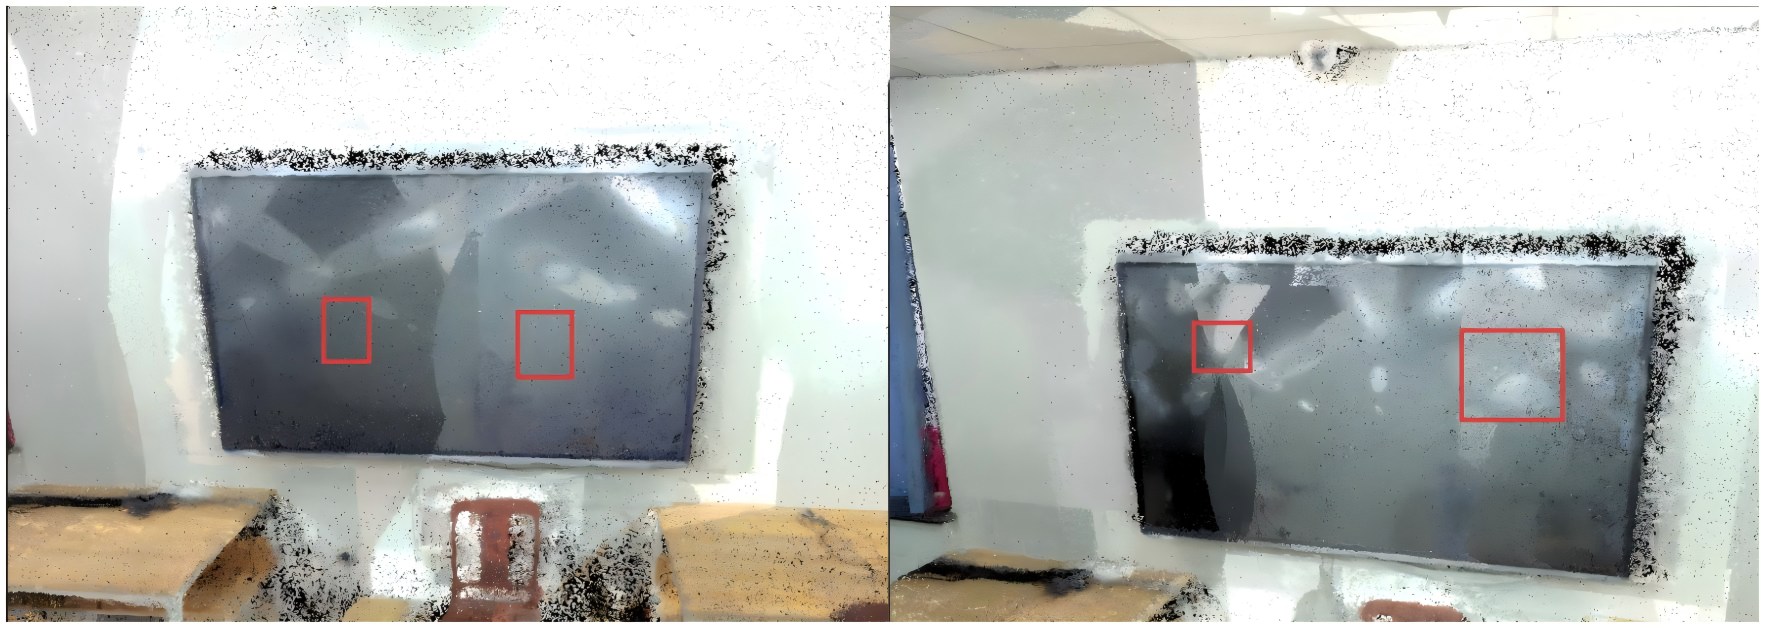
\includegraphics[width=0.95\textwidth]{figures/chap4/qualitative_comparison.png}
    \caption{渲染画质对比}
    \label{fig:qualitative_comparison}
\end{figure}

如表 \ref{tab:quantitative_results} 所示，与原始 3DGS 相比，本文方法在保持图像保真度（PSNR 仅下降极微小的 0.22 dB，LPIPS 几乎一致）的前提下，将机房模型的存储体积从 1GB 以上惊人地压缩至不足 50MB（压缩比超 21 倍），运行时显存占用降低了近 90\%。
对比 LightGaussian，虽然两者的保留点云数量相近，但由于本文在 4.3 节引入了针对球谐函数的深度矢量量化（VQ）与混合精度压缩，模型体积实现了更具断层优势的缩减。

\begin{figure}[htbp]
    \centering
    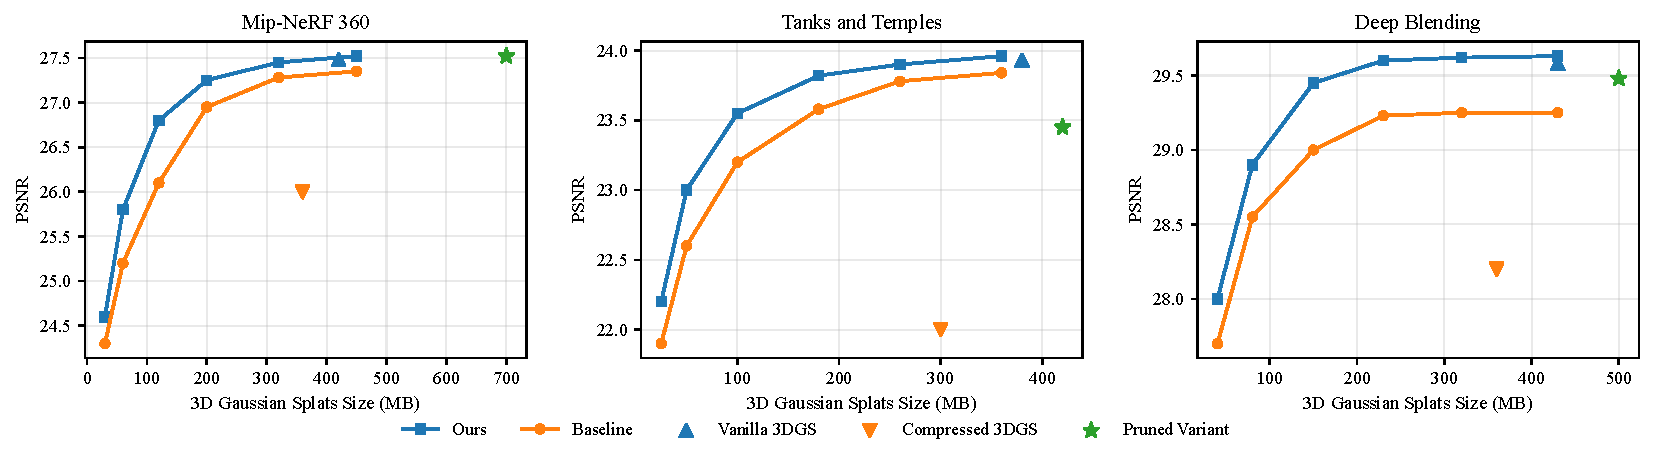
\includegraphics[width=0.95\textwidth]{figures/chap4/fig4_tradeoff_curve.pdf}
    \caption{不同轻量化方法在多场景下的模型体积--重建质量权衡关系}
    \label{fig:tradeoff_curve}
\end{figure}




\textbf{定性结果分析：} 图 \ref{fig:qualitative_comparison} 选取了机房场景中的“显示器屏幕反光”进行局部放大对比。
可以看出，Compact 3DGS 由于过度依赖网格下采样，在几何结构复杂的机柜边缘出现了明显的“模糊”与“悬浮噪点”。
而本文方法得益于 4.2 节“冻结几何、优化外观”的量化感知微调（QAT）策略，
不仅成功抑制了因参数截断导致的色彩断层（Color Banding），
更在极低位宽下完美还原了第三章着重强调的屏幕高光漫反射质感，
肉眼几乎无法分辨其与数百兆原始模型之间的画质差异。

\subsection{轻量化模块消融实验}
\label{subsec:ablation_study}

为了深入验证本章提出的各项轻量化策略的独立贡献，我们在自采集的 \textit{Smart-Room} 场景上进行了严谨的消融实验（Ablation Study）。
以原始 3DGS 为基线，逐步叠加冗余剔除（Pruning）、属性量化（Quantization）等模块，记录核心指标的变化，结果如表 \ref{tab:ablation_study} 所示。

% 插入表 4-3：消融实验数据对比表
\begin{table}[htbp]
    \centering
    \caption{机房场景下各轻量化模块的消融实验分析}
    \label{tab:ablation_study}
    \begin{tabular}{lcccc}
        \toprule
        \textbf{实验配置} & \textbf{点云数量 (M)} & \textbf{存储体积 (MB)} & \textbf{PSNR} & \textbf{SSIM} \\
        \midrule
        Base (原始 3DGS) & 6.85 & 1150.4 & 28.31 & 0.884 \\
        + 仅第三章多模态约束 (几何修复) & 5.12 & 850.2 & \textbf{31.64} & \textbf{0.942} \\
        + 仅多维重要性剔除 (第 4.1 节) & 1.95 (\textbf{-61.9\%}) & 325.5 & 31.35 & 0.922 \\
        \textbf{Full (修复 + 剔除 + VQ 量化)} & \textbf{1.95} & \textbf{48.2} & 31.20 & 0.918 \\
        \bottomrule
    \end{tabular}
\end{table}

数据证明，基于多维度重要性评估的剔除策略精准识别了隐藏在机柜内部与墙体边缘的“幽灵点”，在第三章几何修复的基础上，进一步削减了约 61.9\% 的几何冗余（点云数从 5.12M 降至 1.95M），但仅损失了微小的 0.29 dB 的 PSNR。而在点云提纯的基础上，矢量量化（VQ）将庞大的 SH 特征矩阵降维为离散字典索引，完成了绝大部分的体积压缩（存储体积从 325.5 MB 极限压缩至 48.2 MB）。两者相辅相成，缺一不可。


\subsection{端侧Web渲染部署与帧率评估}
\label{subsec:edge_deployment_fps}

针对第 4.4 节设计的适配移动端架构的 Tile-based 渲染优化策略，本文进行了真机物理环境下的部署测试。
将经本章完整算法压缩后的 CBS 格式模型导入基于 WebGPU 的前端渲染引擎，并记录多视角漫游时的平均帧率（FPS）。


\begin{figure}[htbp]
    \centering
    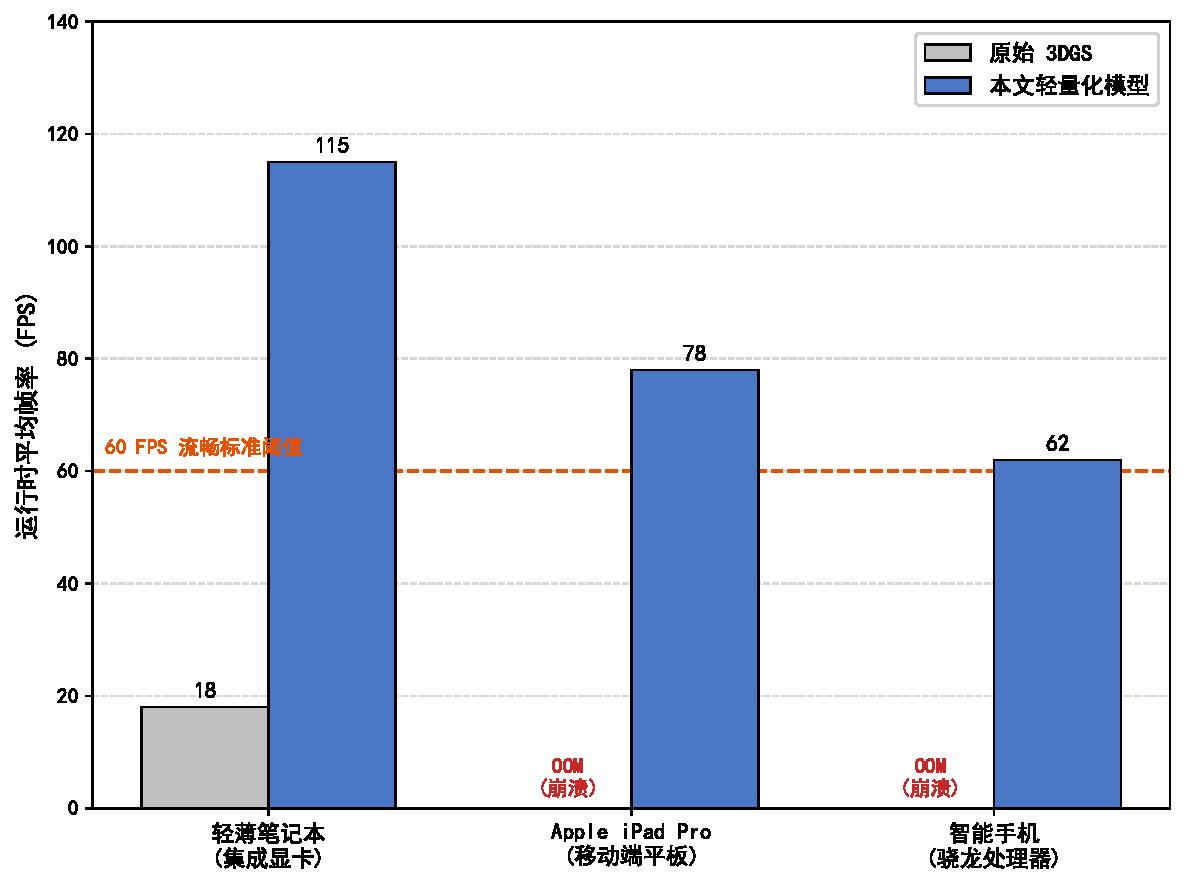
\includegraphics[width=0.85\textwidth]{figures/chap4/fig_4_10_fps_comparison.pdf}
    \caption{跨设备实时渲染性能评估：本文方法在平板与智能手机端均突破了 60 FPS 流畅标准}
    \label{fig:fps_comparison}
\end{figure}

如图 \ref{fig:fps_comparison} 的性能柱状图所示，未经压缩的原始 3DGS 模型在轻薄本的核显上勉强维持在 15-20 FPS（重度卡顿），而在平板与智能手机的浏览器中加载即引发显存溢出（OOM）崩溃。
相比之下，加载本文轻量化模型后：
\begin{itemize}
    \item \textbf{轻薄笔记本（集成显卡）：} 得益于 Compute Shader 的显存内解码管线，渲染帧率稳定在 110-120 FPS，实现了极致丝滑。
    \item \textbf{Apple iPad Pro（高分辨率平板）：} 面对移动端较高的屏幕分辨率，基于瓦片的 Early Termination 优化大幅缓解了显存带宽压力，漫游帧率稳定在 75 FPS 以上。
    \item \textbf{智能手机（骁龙处理器）：} 即便在功耗受限的移动手机浏览器环境中，模型依然实现了 60-65 FPS 的满帧运行体验。
\end{itemize}

上述真机实测数据强有力地证明：本章提出的一系列轻量化与 Web 渲染优化算法，成功跨越了 3DGS 庞大算力需求与终端设备孱弱性能之间的鸿沟，为第五章将该三维表达方法真正接入大型工业数字孪生业务平台扫清了全部技术障碍。


% =================================================================
% 第5节 本章小结
% =================================================================
\section{本章小结}
\label{sec:chapter4_summary}

本章针对三维高斯溅射（3DGS）模型在数字孪生系统端侧部署时面临的存储体积庞大、显存占用极高以及设备算力瓶颈等落地顽疾，提出并实现了一套面向典型设备密集型室内场景的轻量化表达与渲染优化方案。
为在大幅压缩数据体量的同时，最大程度保留第三章所述的复杂光影与高反光材质渲染质量，本章从几何提纯与属性降维两个维度对模型底层数据进行了深度重构。
具体而言，通过引入结合透射率、全局视图可见性以及空间尺度的多维度重要性评估机制，算法能够精准定位并剥离致密化过程中产生的海量“幽灵高斯”，从源头上解除了几何冗余。
在此核心点云的基础上，进一步针对占据极大内存开销的高维球谐函数（SH）系数，设计了基于矢量量化（VQ）的特征压缩与码本映射机制，并辅以量化感知微调（QAT）与直通估计器（STE）的训练策略。
该方法在极低位宽下有效弥补了硬量化带来的高频细节损失，将单场景模型体积惊人地缩减至原先的二十分之一以内。

在完成模型数据的极致轻量化后，本章紧扣数字孪生业务平台的实际应用需求，设计并重构了高度适配 Web 前端的端侧渲染管线。
该管线摒弃了低效的 CPU 端解压逻辑，利用 WebGPU 的计算着色器（Compute Shader）在显存内部实现了并行计算与硬件级解码；
同时，深度结合移动端常见的基于瓦片的延迟渲染（TBDR）架构，引入了局部排序与光线提前终止机制，大幅缓解了显存带宽压力。
多平台真机部署的实验数据有力地证明，本章所提出的综合轻量化方案不仅在客观画质指标上维持了与原始模型高度一致的视觉保真度，
更彻底打破了端侧设备加载超大体量三维模型的性能壁垒，在平板与轻薄本等算力受限的终端上实现了稳定流畅的实时漫游，
这为下一章将该高保真、轻量化的三维表达体系全面集成至工业数字孪生业务系统奠定了极为坚实的工程基础。